\section{Interpretability of Failure Cases} 
% \todo{Run experiments and pick failure cases: Extreme occlusion etc. Show a failure case of our method, demonstrating how easy it is to identify and explain/interpret.}
%
\subsection{Visualization}
Being able to visualize the reconstructed objects allows us to reason about failure cases. For example, in scene \textbf{(e)} in Fig.~\ref{fig:interpretability}, we see that the initial object significantly overlaps with the background asphalt in the shadow region, causing the reconstructed car to erroneously generate a darker gray color. Thus, not only does our method allow us to reason about failure cases, but it also identifies ways in which our representation model can be modified to rectify such failures. For example, a generative object model with an additional component that can model different lighting conditions to account for shadows might allow us to identify and reconstruct cars in varied lighting conditions, including shadows. This can guide future work for perception tasks through inverse rendering. \hspace*{\fill} \\


\subsection{Analysis}
Next, we analyze common failure cases using the pre-trained generator as an object prior in the presented tracking method. The visualizations allow us to assess the types of cases where this pipeline fails to track objects. Common failure cases we observed are listed below, with visualizations of such failure cases shown in Figure \ref{fig:interpretability}. We describe the cases corresponding to the rows (a-d, see figure labels) as follows:

\begin{enumerate}[label=(\alph*)]
    \item The apparent darker color of the car due to \textbf{shadows} often causes the predicted object color to be darker than the color a human would perceive the car as. In the presented case on the right, the white car is completely occupied by the shadow of the neighboring truck. While the human visual system perceives the color of the car as white, the numerical RGB value in the image is closer to grey/black. This causes the predicted embedding corresponding to the texture of the object to represent the darker color. This might cause the tracking to fail due to incorrect matching of corresponding objects in consecutive frames with and without shadows. \\
    
    \item Extreme \textbf{reflections} on the car due to the lighting conditions cause the model to try to model the RGB color of the reflection by erroneously modifying the texture of the generated object. Here, clouds in the sky are reflected as white spots on the hood and windshield of the red car, causing reflection and changes of these, influencing the generated texture as white spots. Future work that includes explicit models of BRDF would be beneficial in mitigating this class of failure modes. \\
\end{enumerate} \\

\begin{enumerate}[label=(\alph*)]\setcounter{enumi}{2}
    \item In addition to visualization and interpretation of the object prior more traditional aspects of the perception pipeline, such as ID-switches through \textbf{occlusion} in multi-object tracking scenarios can be observed. Here, the first object in the background (green box, $t_0$) is misidentified as the second object (green box, $t_1$). Such visualization allows further reasoning about the full pipeline. \\
    
    \item Camera \textbf{obstructions} and extreme local \textbf{lighting}, such as in raindrops, lens flares, and bright lights, cause our method to erroneously predict the shape and texture of many cars to match the perceived shape of the car, causing matching to fail. \\
    
    \item Inaccuracies in the predicted pose cause the predicted car in front to not perfectly align with the observed car patch, causing there to be an overlap between the predicted car and the immediate surroundings in the observed image, here the asphalt. Since only information on the detection is available, the color of the optimized object tends to be predicted gray (since the road is gray, and so the optimized texture embedding is closer to gray).
\end{enumerate}

% \begin{wrapfigure}{r}{0.6\linewidth}
\begin{figure}[bt!]
	\centering
\resizebox{1.\linewidth}{!}{
\renewcommand{\arraystretch}{0.5}
\begin{tabular}{@{}c@{\hskip 0.05cm}c@{\hskip 0.05cm}c@{\hskip 0.05cm}c@{}}
		\space
            &
		{\huge Input $t_0$}&
		{\huge Tracked $t_0$}&
		{\huge Tracked $t_1$}&
		% {\small Tracked $t_2$}&
		% {\small Tracked $t_3$}\\

   %           \rotatebox[origin=c]{90}{{\large  Similar colored cars}}&
		 % \raisebox{-0.5\height}{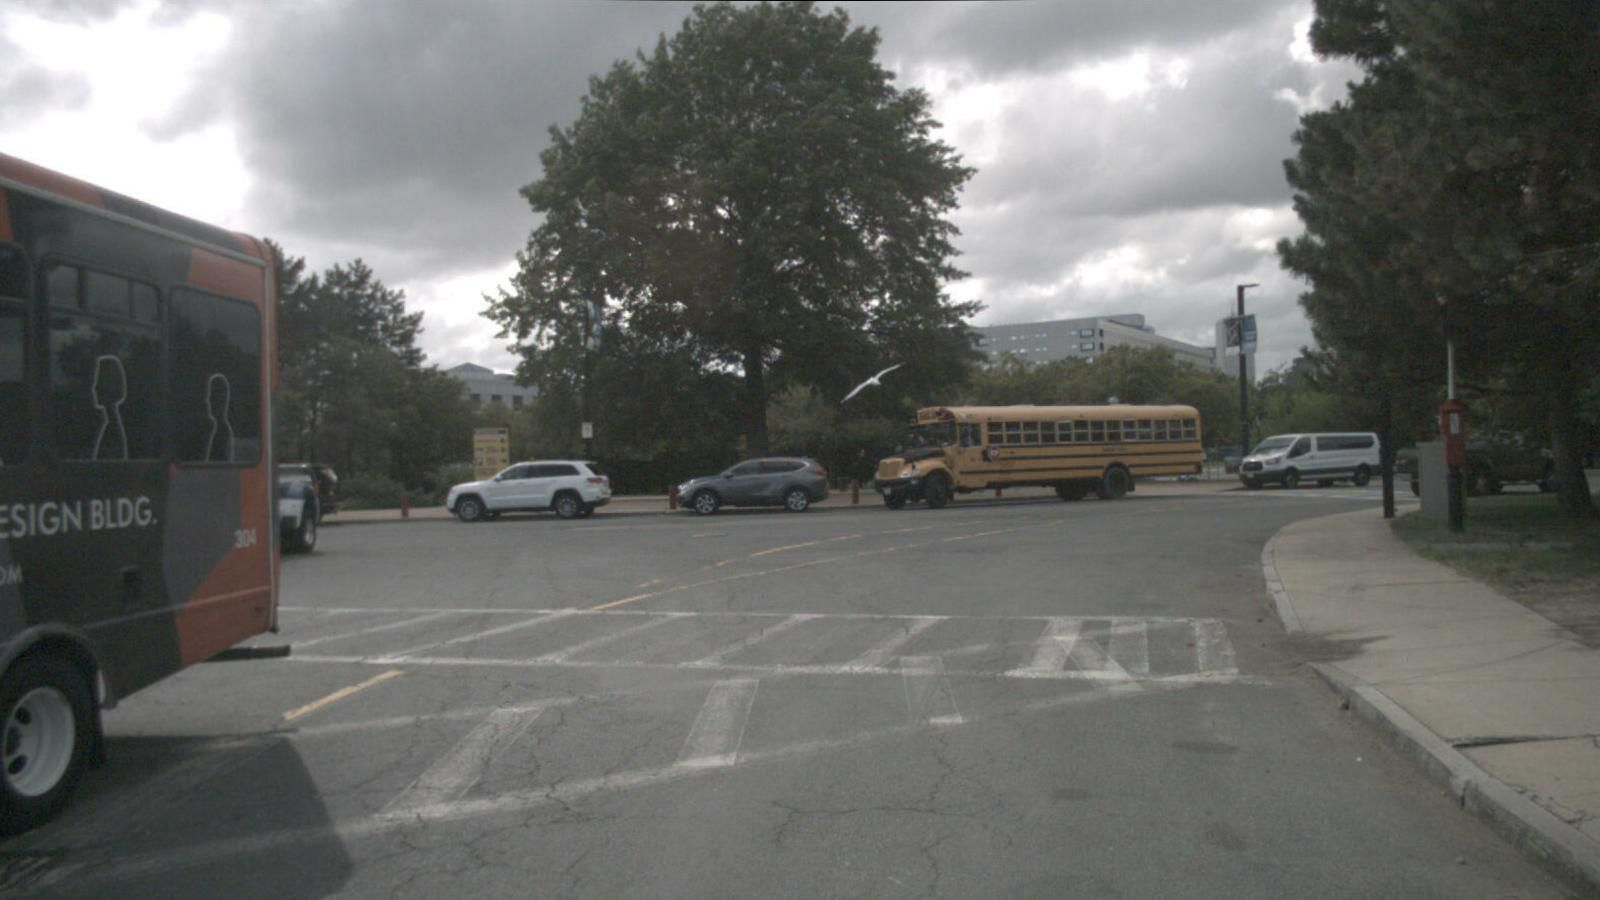
\includegraphics[width=.38\columnwidth, trim={0cm 0cm 0cm 0cm},clip]{fig/additional_nuscenes_results/scene1/26_gt.png}}&
		 % \raisebox{-0.5\height}{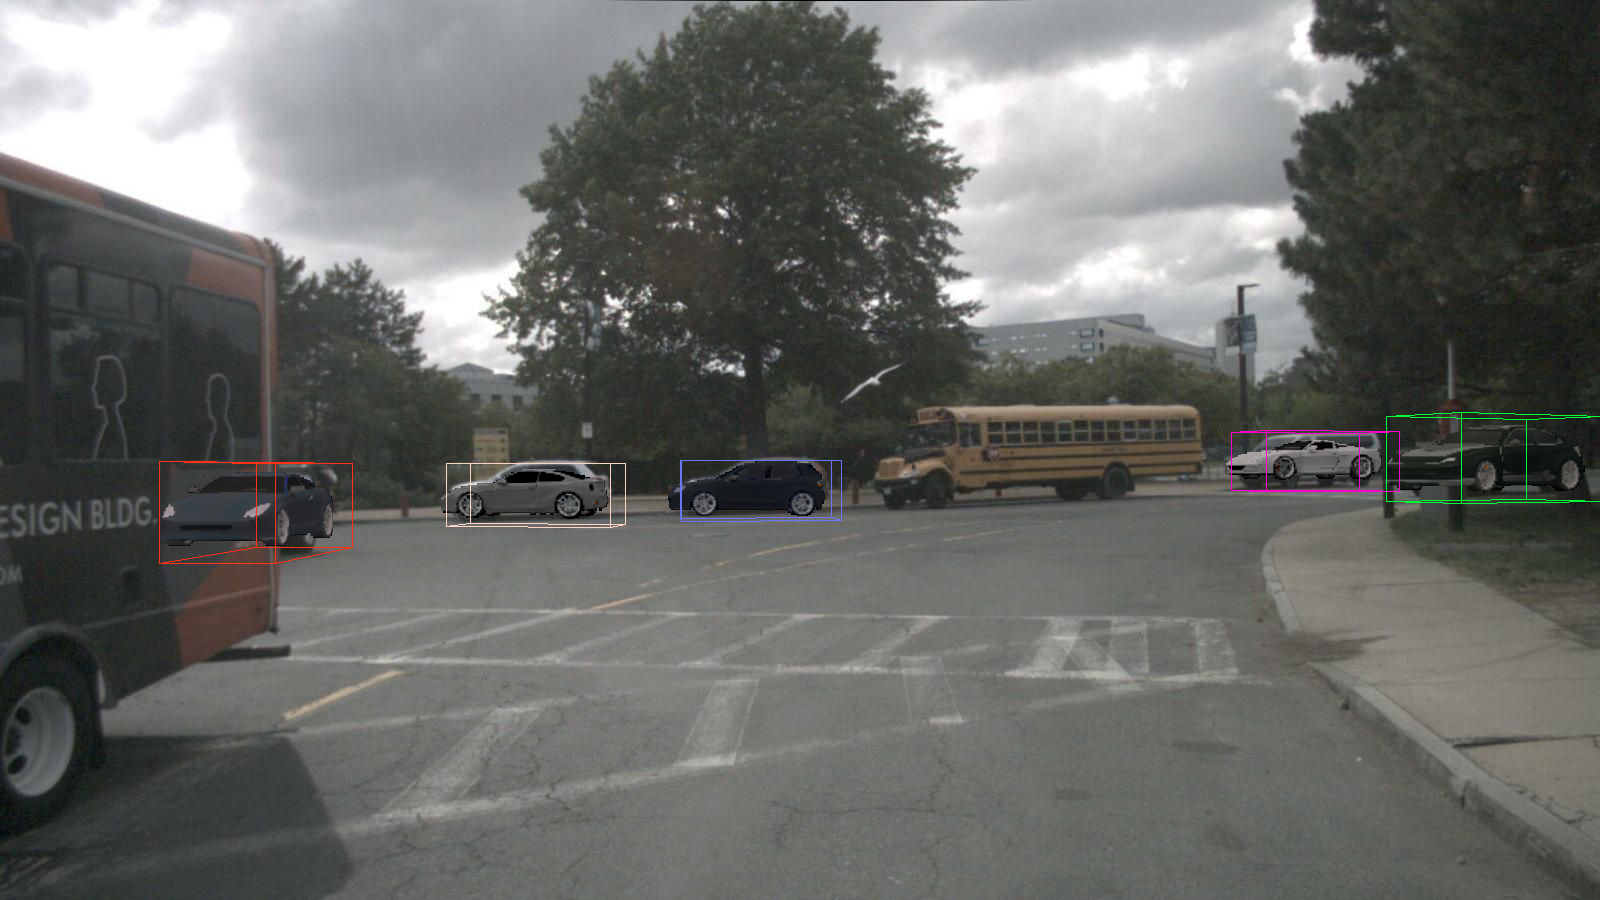
\includegraphics[width=.38\columnwidth, trim={0cm 0cm 0cm 0cm},clip]{fig/additional_nuscenes_results/scene1/26_bbox.png}}&
		 % \raisebox{-0.5\height}{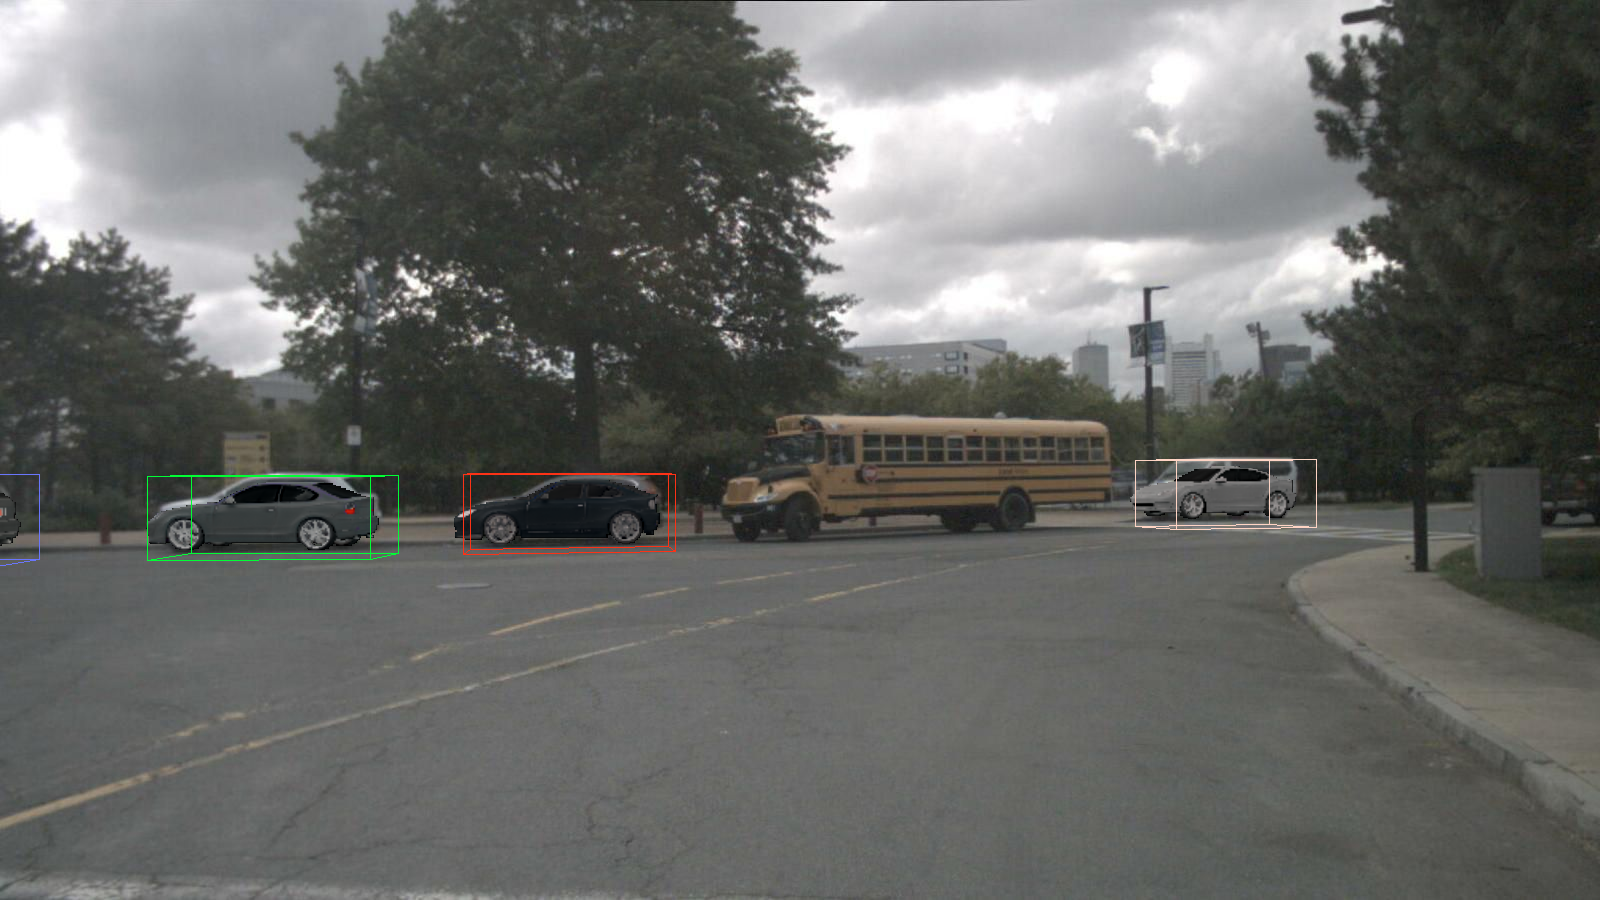
\includegraphics[width=.38\columnwidth, trim={0cm 0cm 0cm 0cm},clip]{fig/additional_nuscenes_results/scene1/28_bbox.png}}&
		 % \raisebox{-0.5\height}{
\includegraphics[width=.38\columnwidth, trim={0cm 0cm 0cm 0cm},clip]{fig/placeholder-img.png}}&
		 % \raisebox{-0.5\height}{
\includegraphics[width=.38\columnwidth, trim={0cm 0cm 0cm 0cm},clip]{fig/placeholder-img.png}}\\[0.95cm]

           \rotatebox[origin=c]{90}{{\Large \textbf{(a)} Shadow}}&
  		\raisebox{-0.5\height}{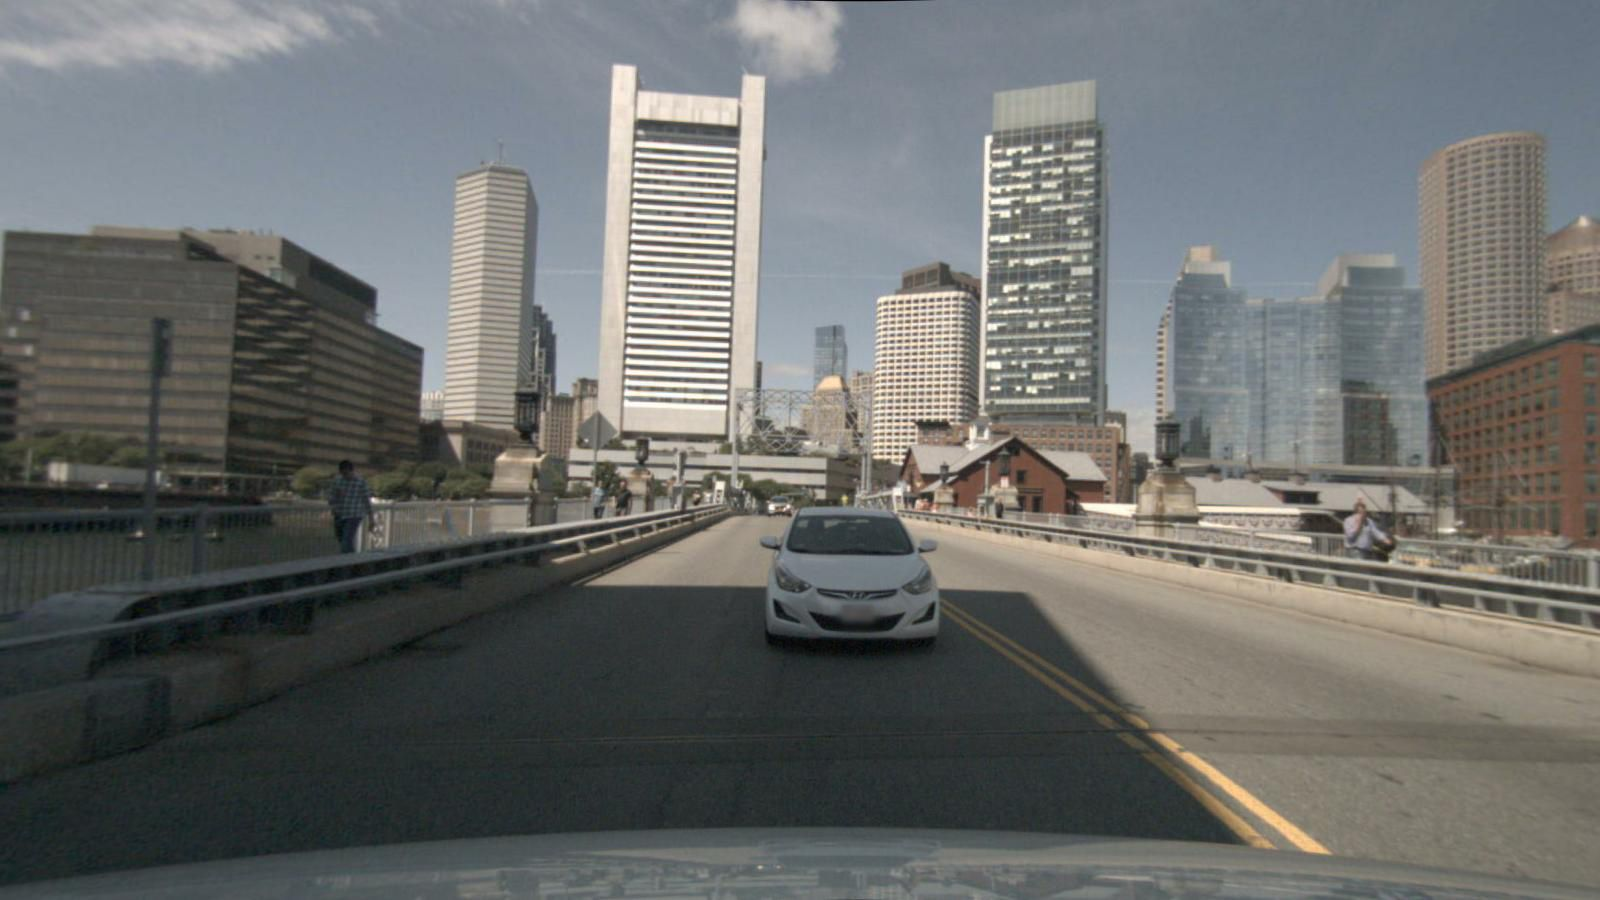
\includegraphics[width=.7\columnwidth, trim={0cm 0cm 0cm 0cm},clip]{fig/additional_nuscenes_results/scene12/gt.png}}&
		\raisebox{-0.5\height}{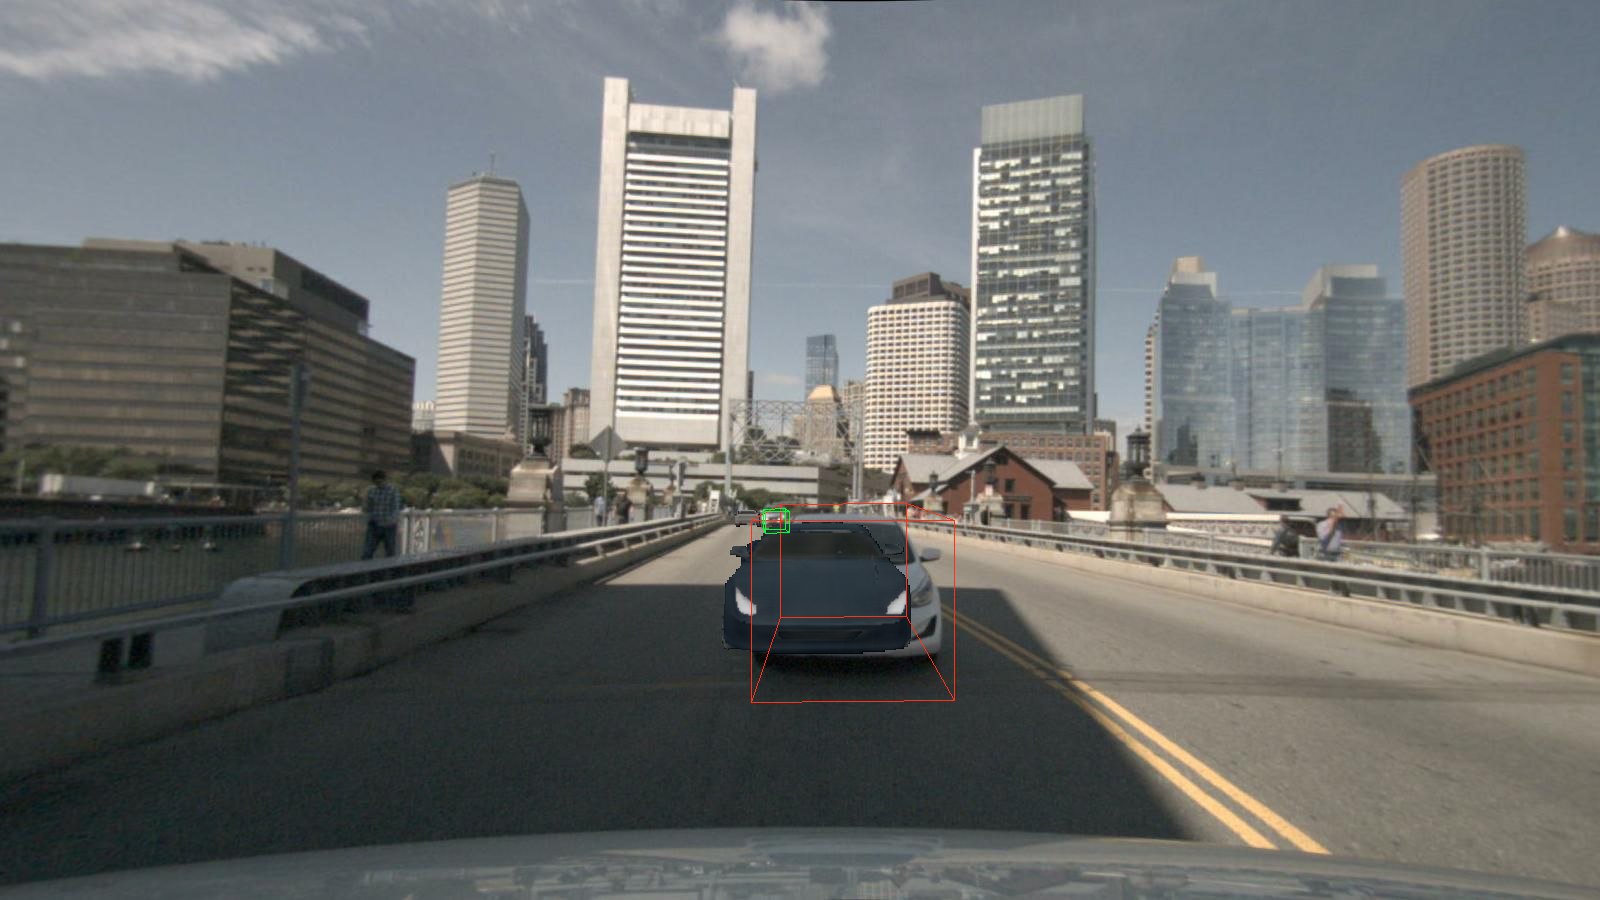
\includegraphics[width=.7\columnwidth, trim={0cm 0cm 0cm 0cm},clip]{fig/additional_nuscenes_results/scene12/21.png}}&
		\raisebox{-0.5\height}{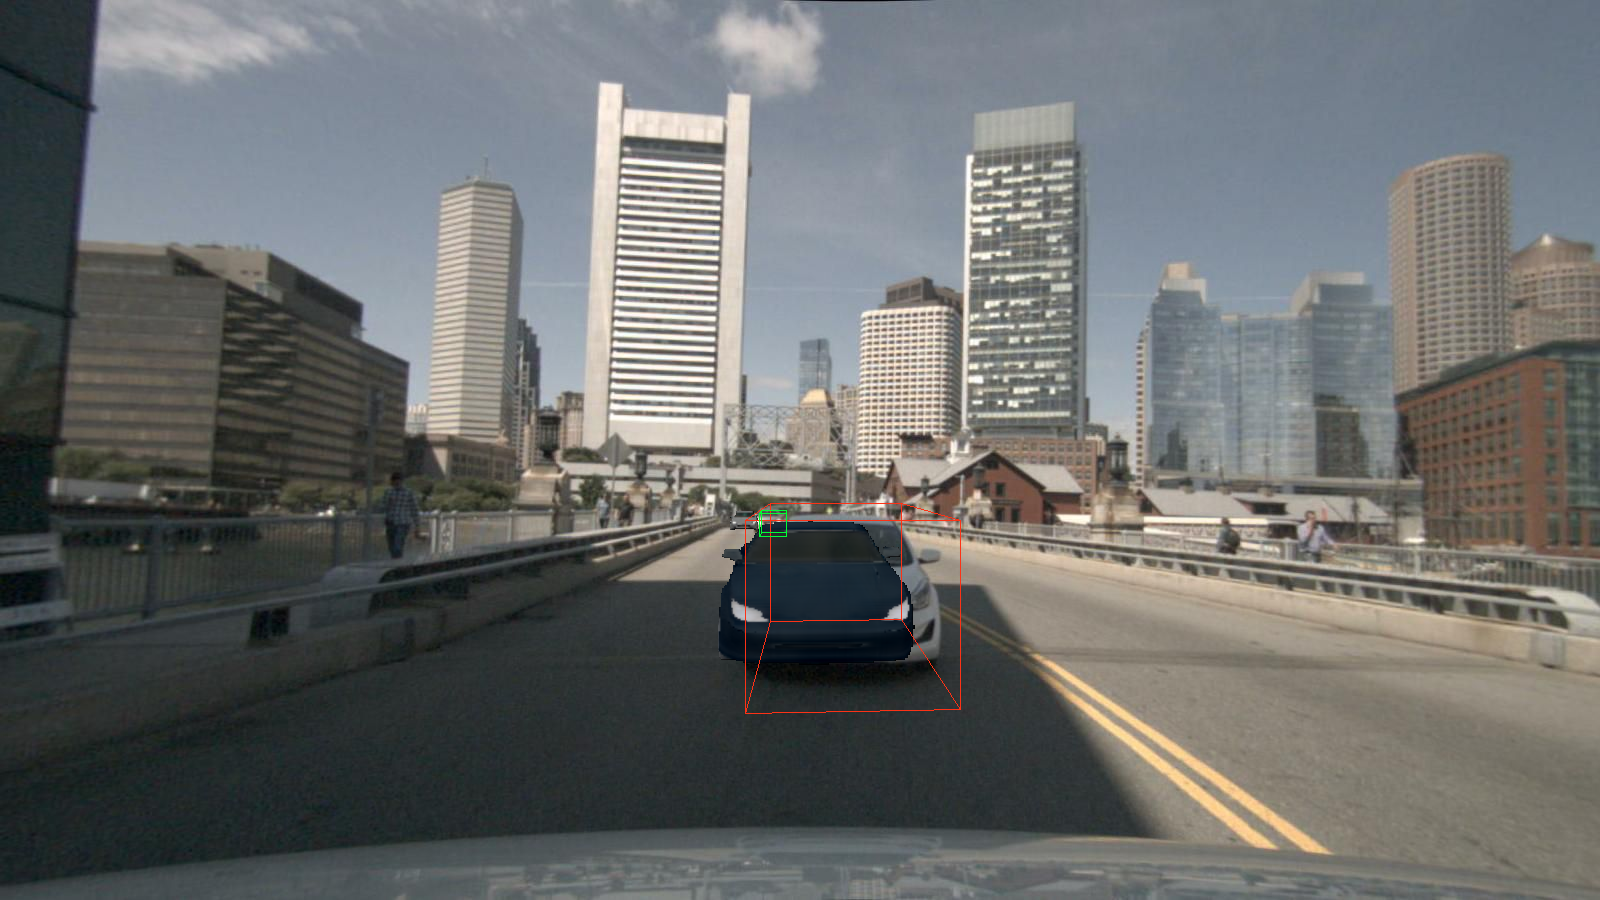
\includegraphics[width=.7\columnwidth, trim={0cm 0cm 0cm 0cm},clip]{fig/additional_nuscenes_results/scene12/22.png}}&
		% \raisebox{-0.5\height}{
\includegraphics[width=.38\columnwidth, trim={0cm 0cm 0cm 0cm},clip]{fig/placeholder-img.png}}&
		% \raisebox{-0.5\height}{
\includegraphics[width=.38\columnwidth, trim={0cm 0cm 0cm 0cm},clip]{fig/placeholder-img.png}}
  \\[0.02cm]

            \rotatebox[origin=c]{90}{{\Large \textbf{(b)} Reflection}}&
  		\raisebox{-0.5\height}{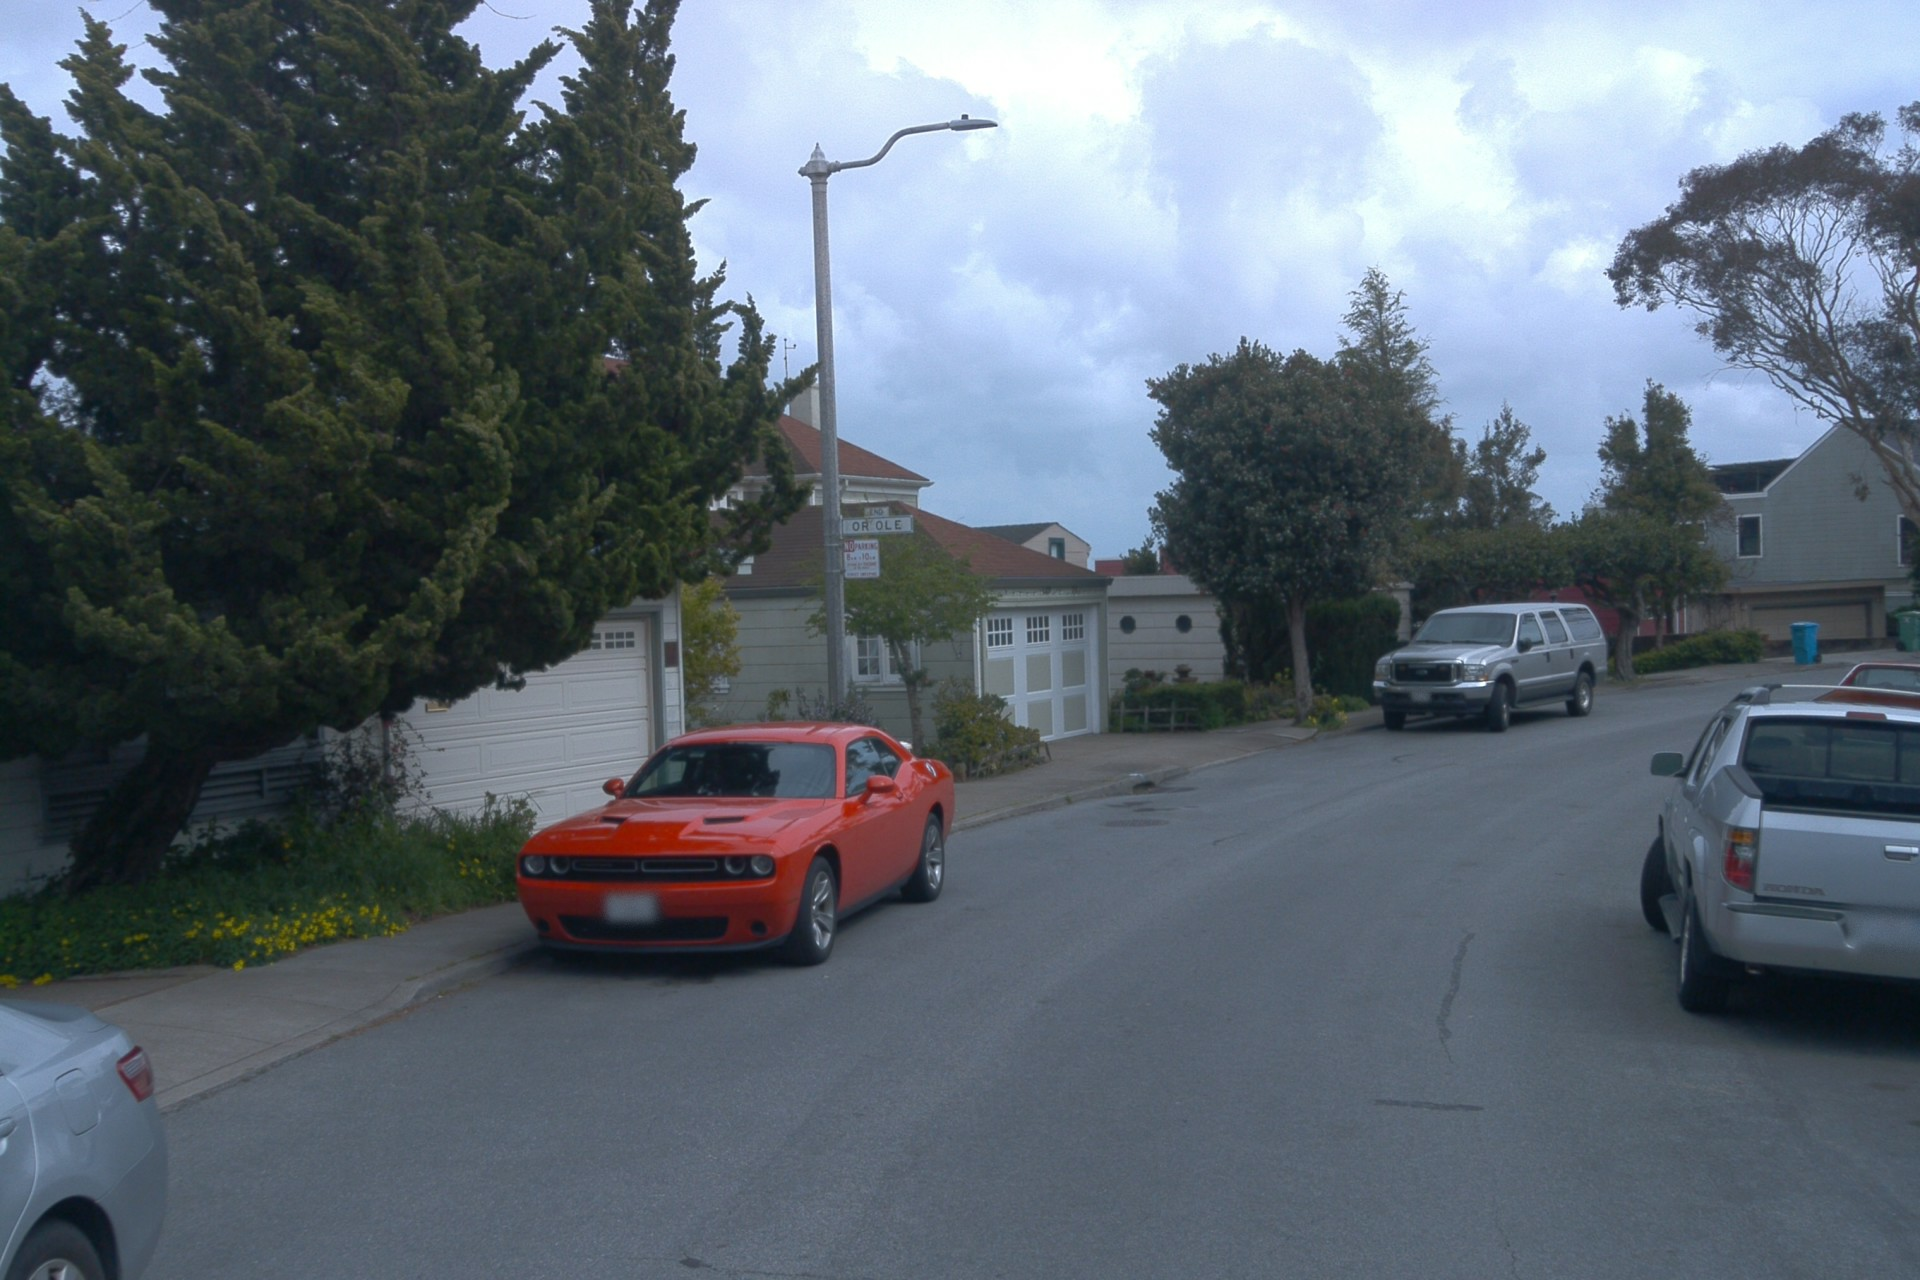
\includegraphics[width=.7\columnwidth, trim={0cm 0cm 0cm 0cm},clip]{fig/additional_waymo_results/scene4/gt_img.png}}&
		\raisebox{-0.5\height}{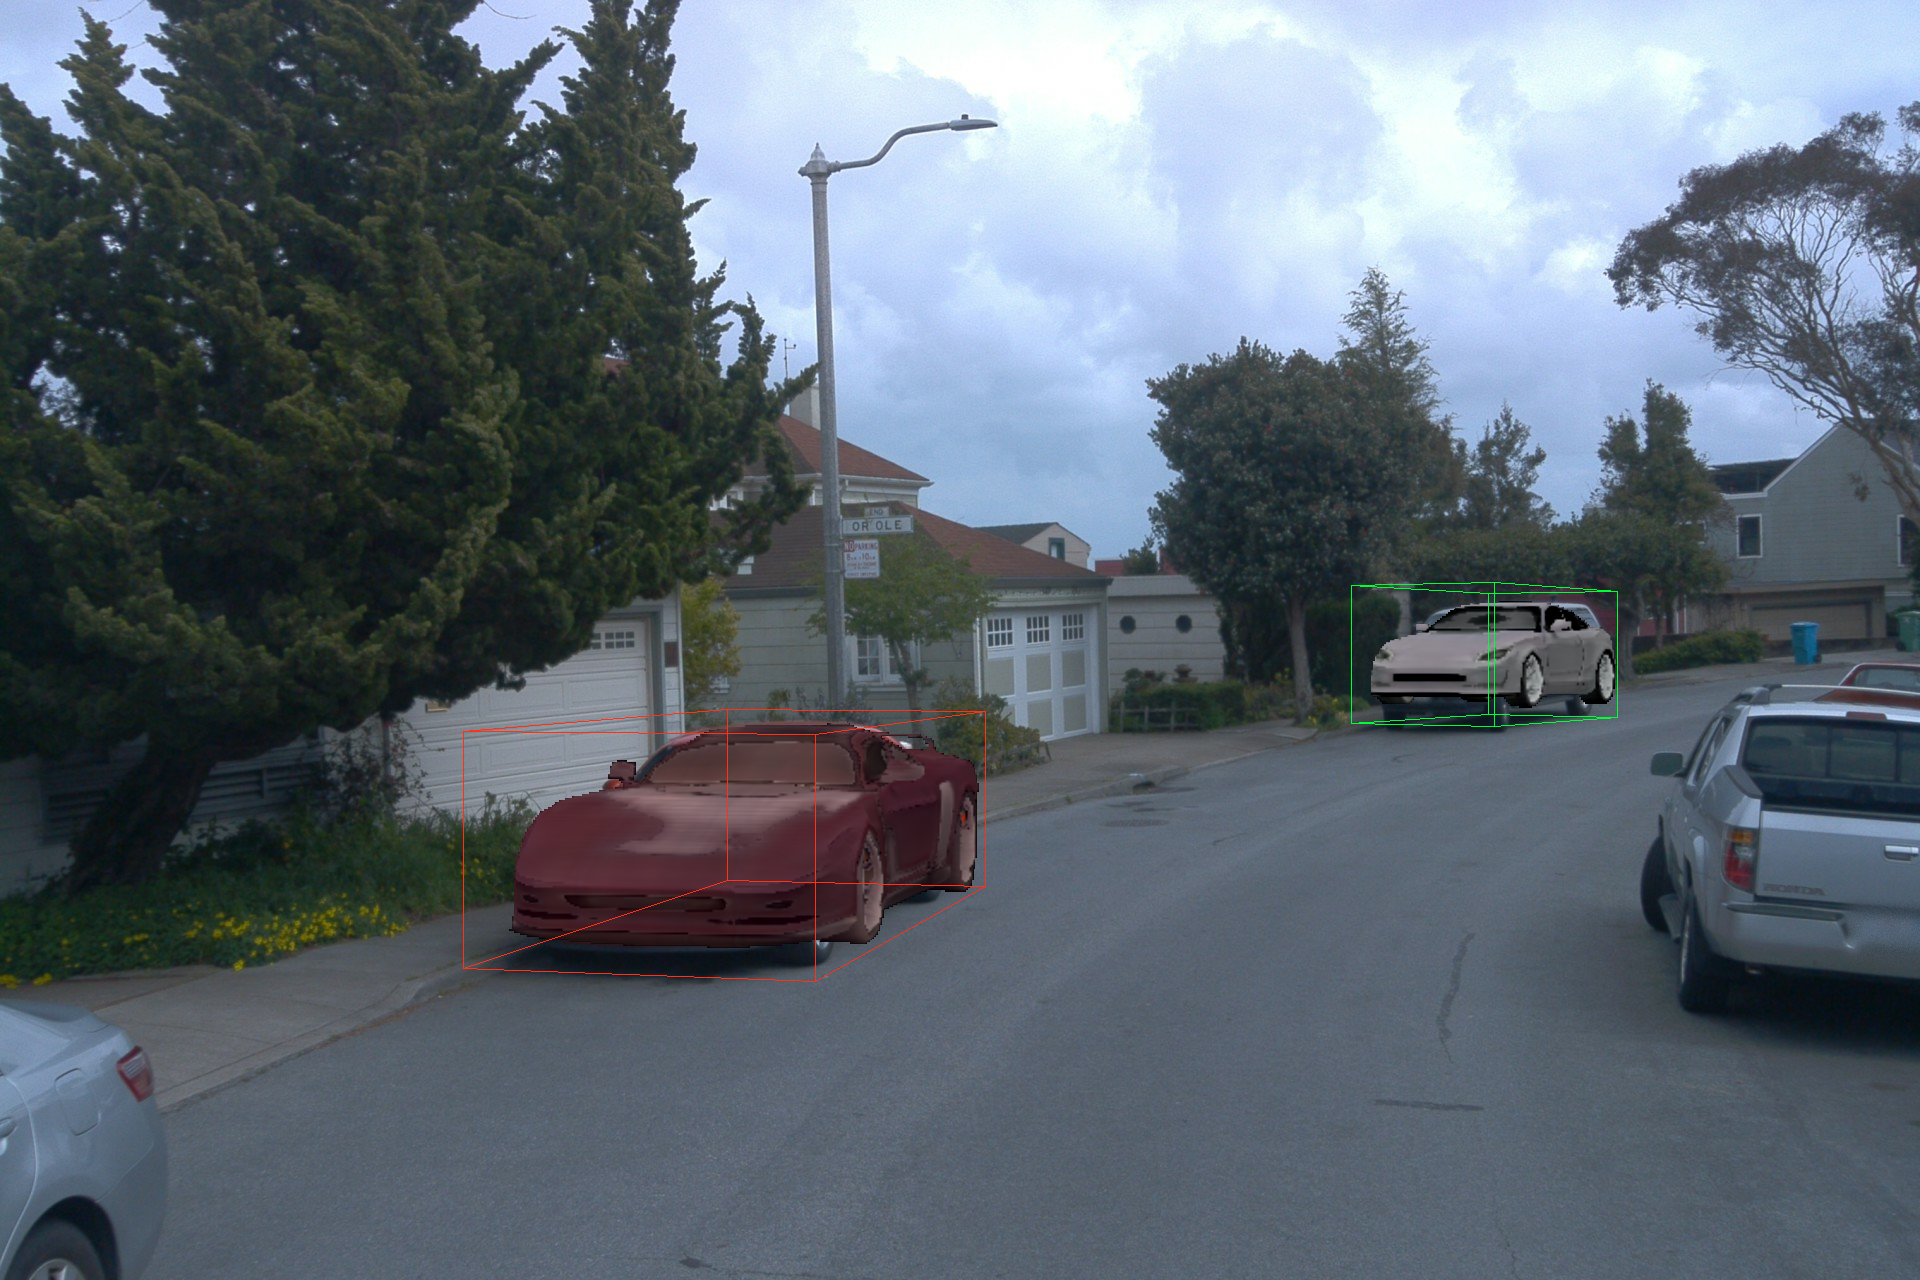
\includegraphics[width=.7\columnwidth, trim={0cm 0cm 0cm 0cm},clip]{fig/additional_waymo_results/scene4/5.png}}&
		\raisebox{-0.5\height}{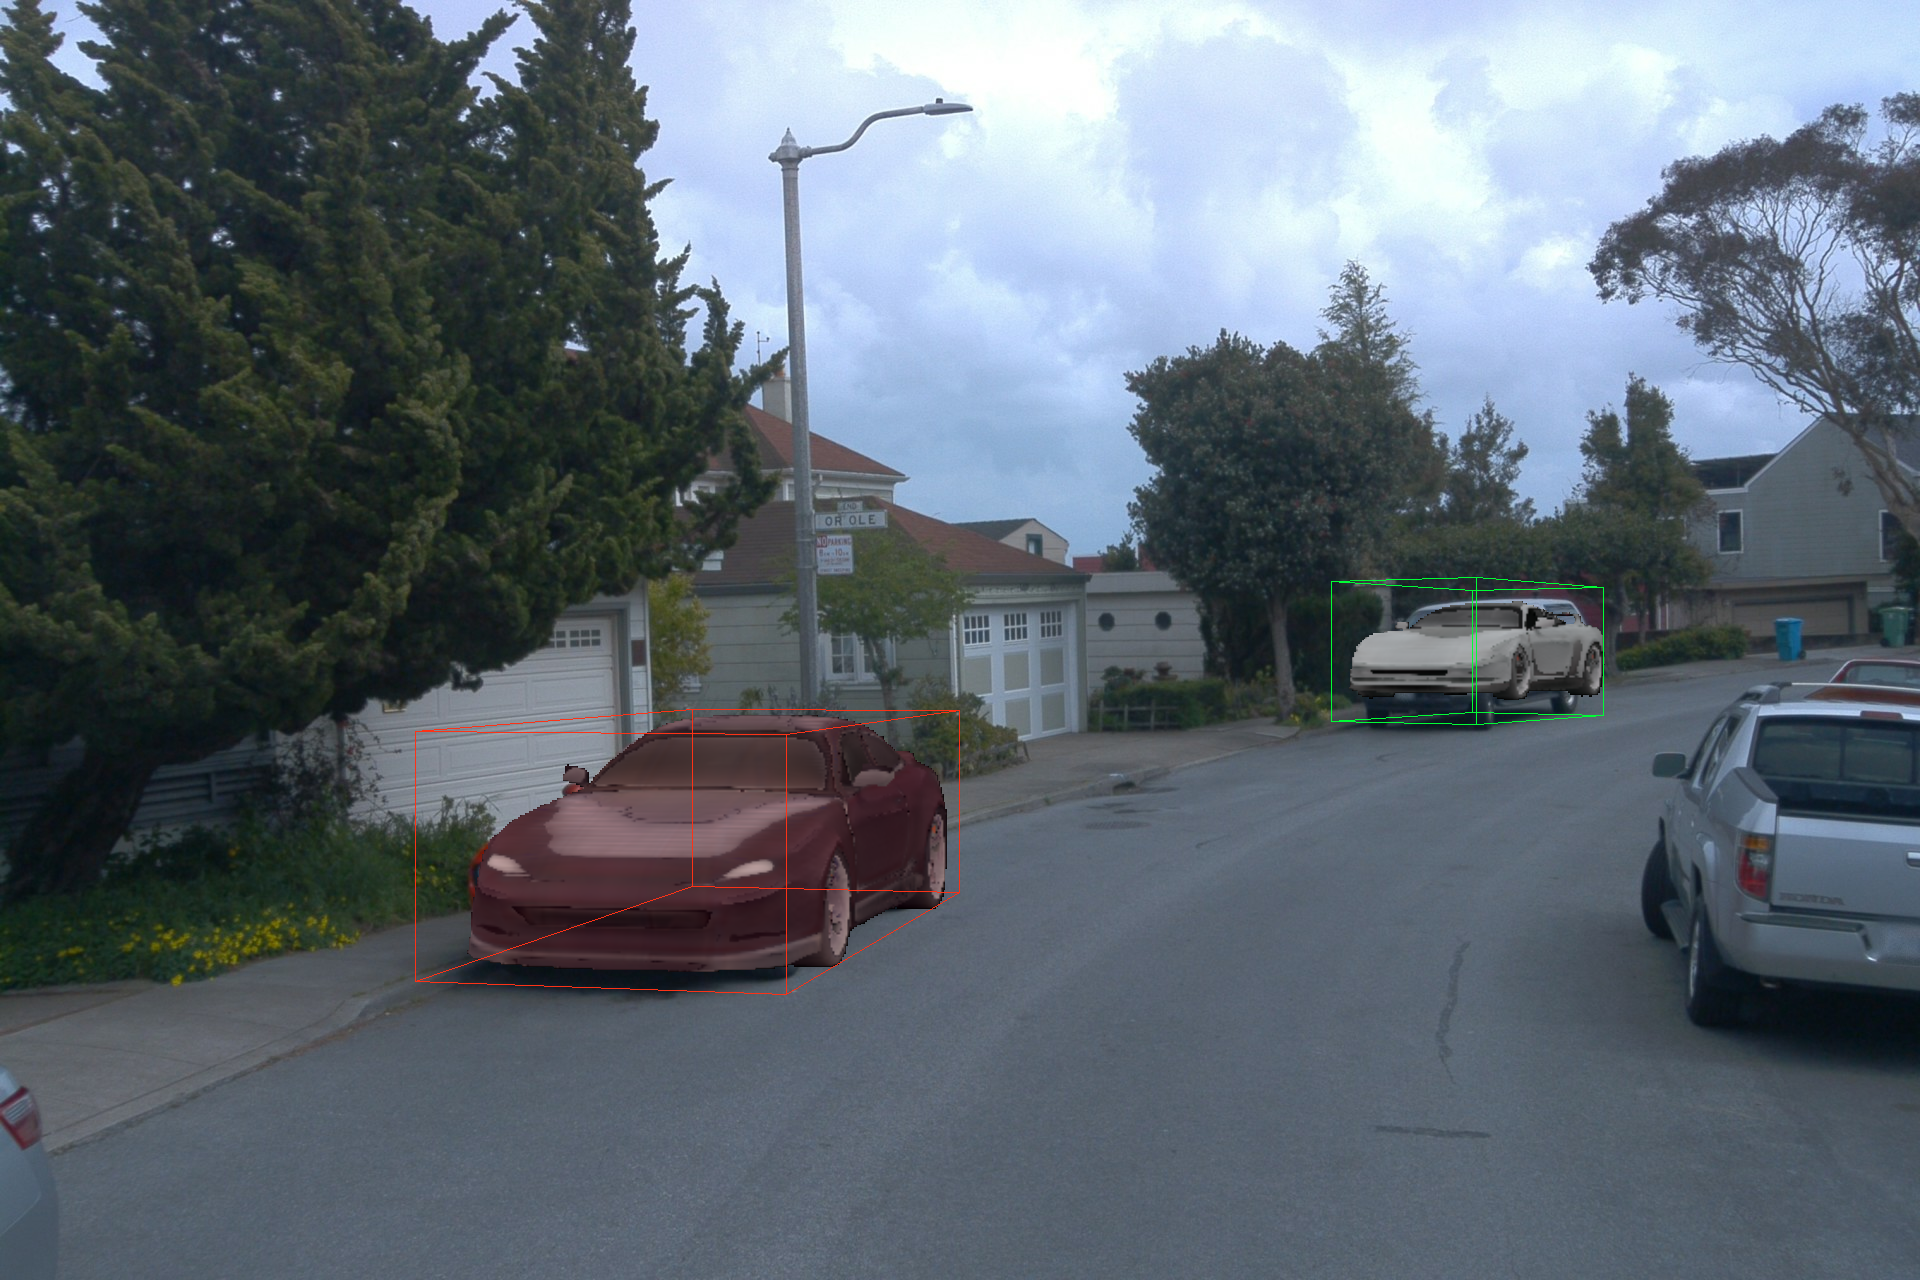
\includegraphics[width=.7\columnwidth, trim={0cm 0cm 0cm 0cm},clip]{fig/additional_waymo_results/scene4/6.png}}&
		% \raisebox{-0.5\height}{
\includegraphics[width=.38\columnwidth, trim={0cm 0cm 0cm 0cm},clip]{fig/placeholder-img.png}}&
		% \raisebox{-0.5\height}{
\includegraphics[width=.38\columnwidth, trim={0cm 0cm 0cm 0cm},clip]{fig/placeholder-img.png}}
  \\[0.02cm]
  
           \rotatebox[origin=c]{90}{{\Large \textbf{(c)} Occlusion}}&
		 \raisebox{-0.5\height}{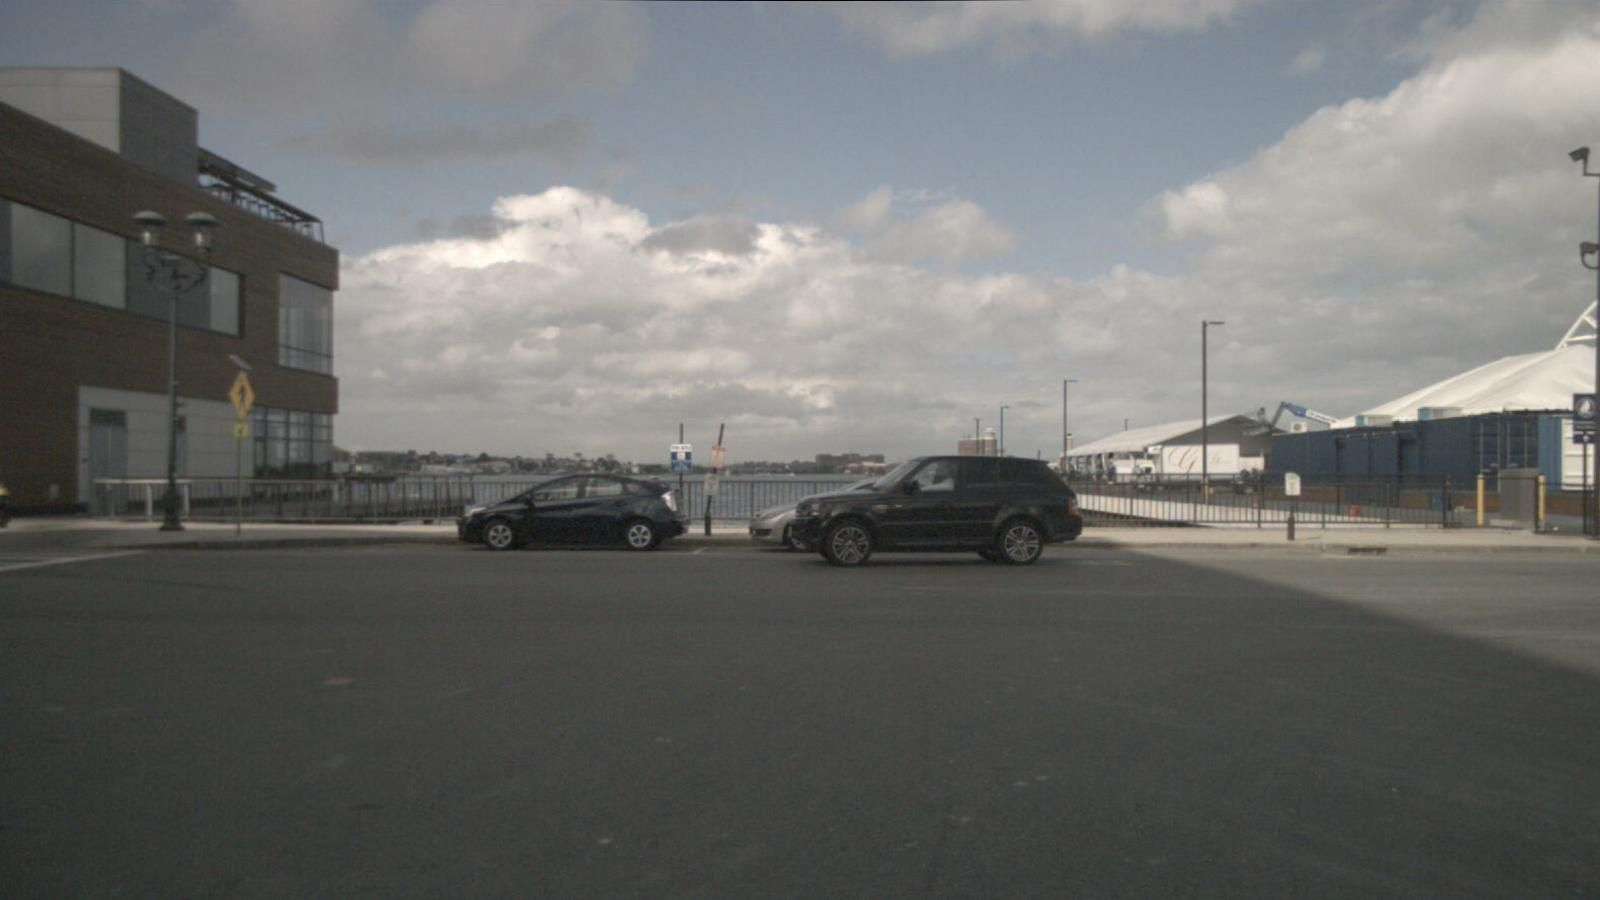
\includegraphics[width=.7\columnwidth, trim={0cm 0cm 0cm 0cm},clip]{fig/additional_nuscenes_results/scene7/0118_4_gt.png}}&
		 \raisebox{-0.5\height}{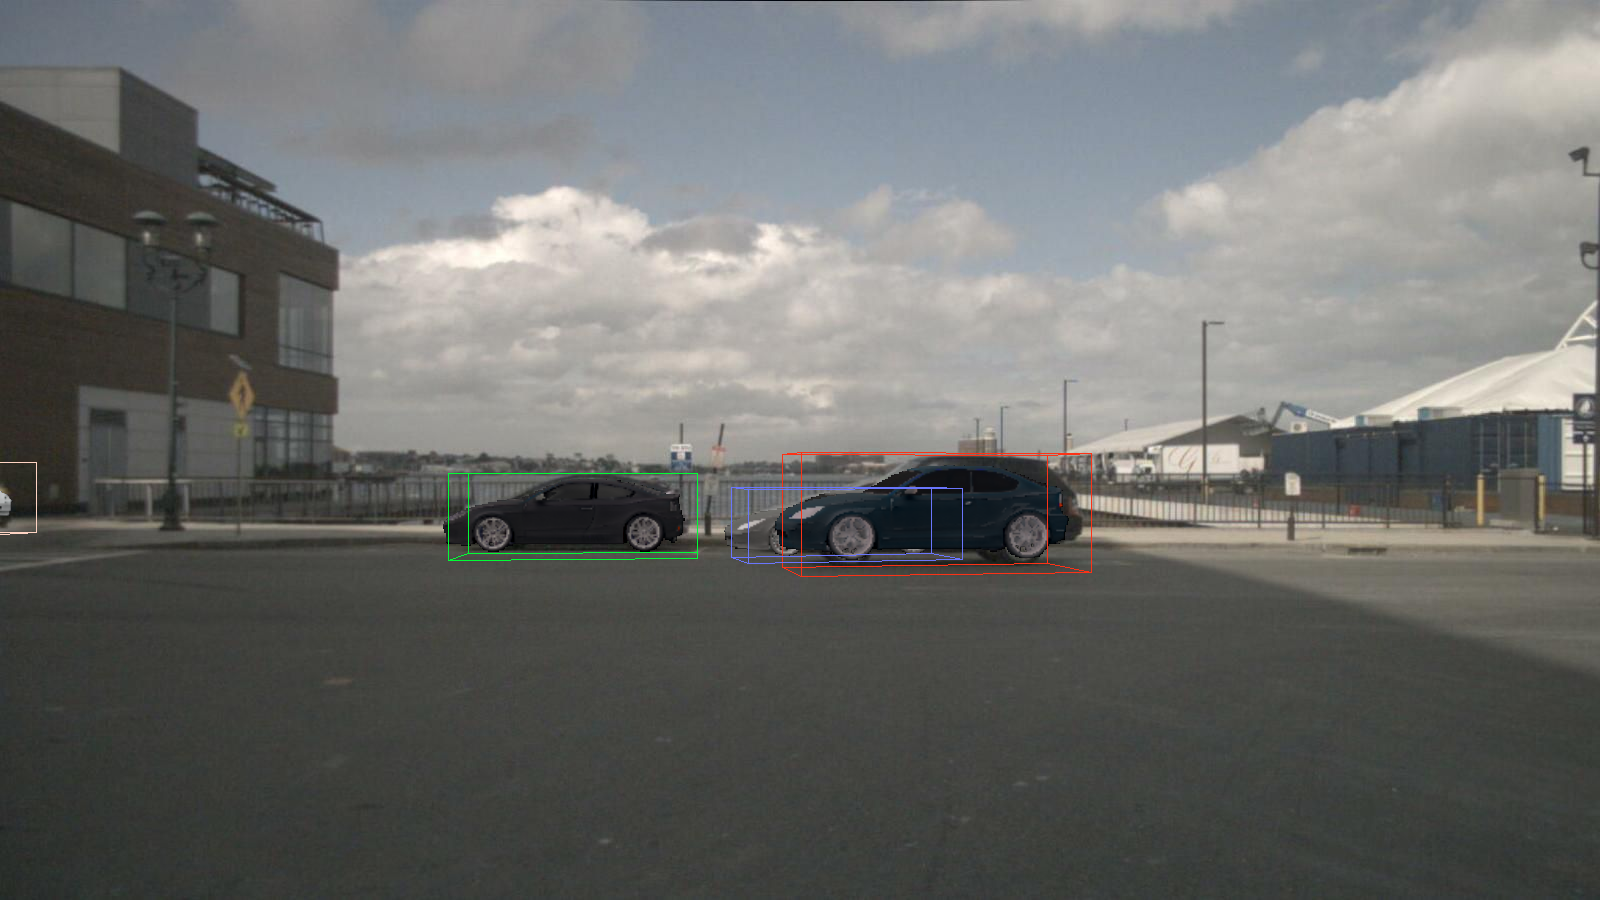
\includegraphics[width=.7\columnwidth, trim={0cm 0cm 0cm 0cm},clip]{fig/additional_nuscenes_results/scene7/0118_4_bbox.png}}&
		 \raisebox{-0.5\height}{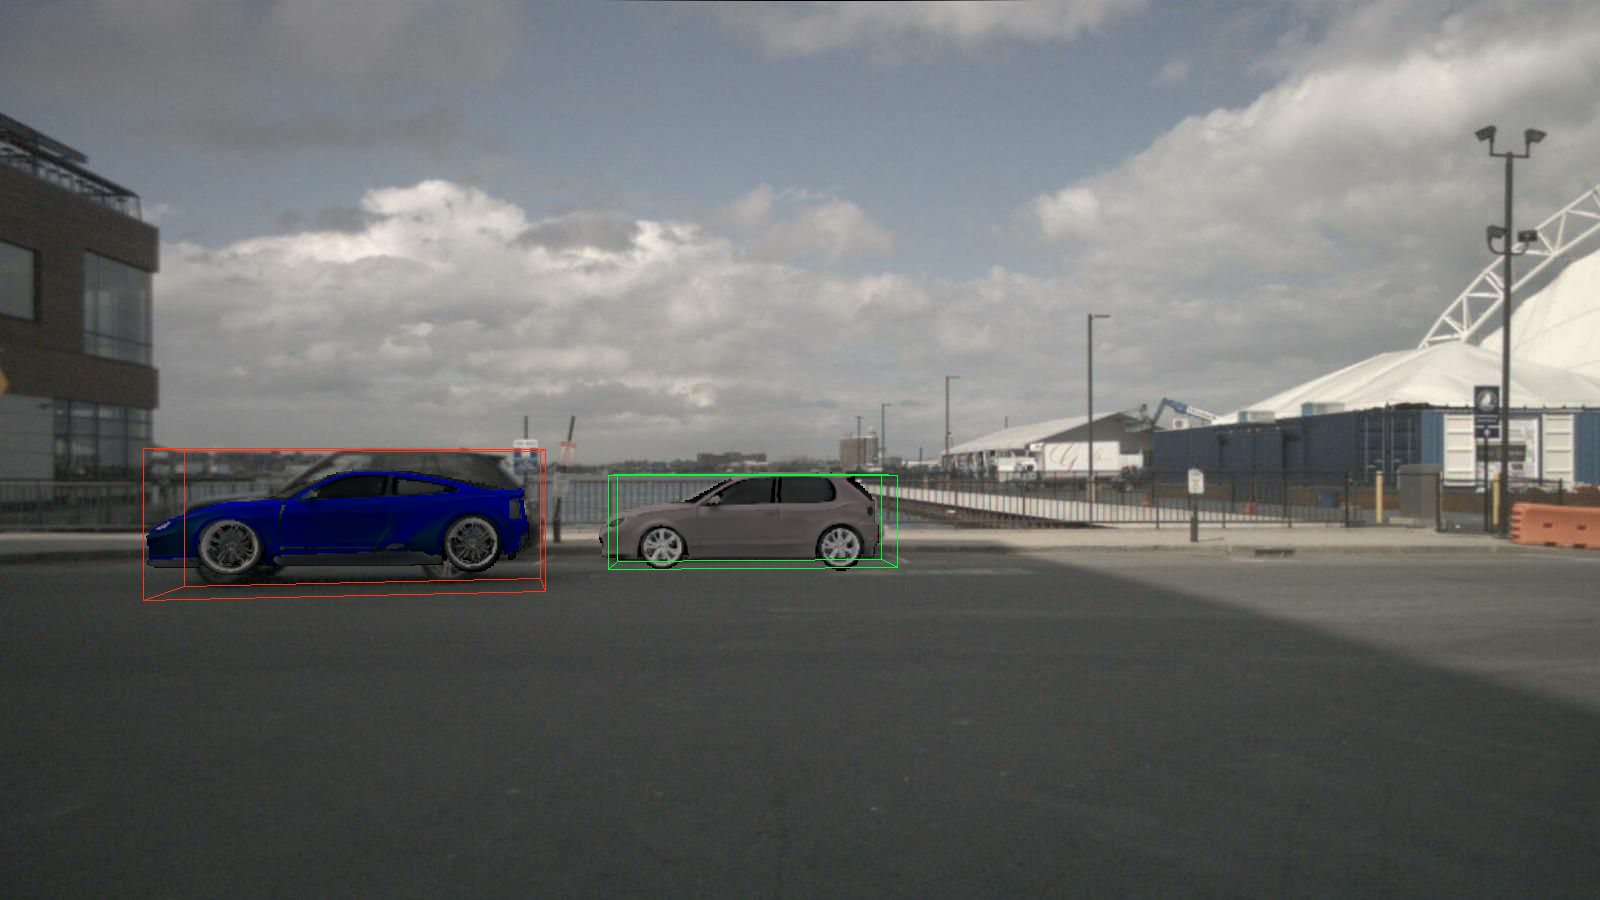
\includegraphics[width=.7\columnwidth, trim={0cm 0cm 0cm 0cm},clip]{fig/additional_nuscenes_results/scene7/0118_6_bbox.png}}&
		 % \raisebox{-0.5\height}{
\includegraphics[width=.38\columnwidth, trim={0cm 0cm 0cm 0cm},clip]{fig/placeholder-img.png}}&
		 % \raisebox{-0.5\height}{
\includegraphics[width=.38\columnwidth, trim={0cm 0cm 0cm 0cm},clip]{fig/placeholder-img.png}}
   \\[0.02cm]
        
        \rotatebox[origin=c]{90}{{\Large \textbf{(d)} Obstruction}}&
		 \raisebox{-0.5\height}{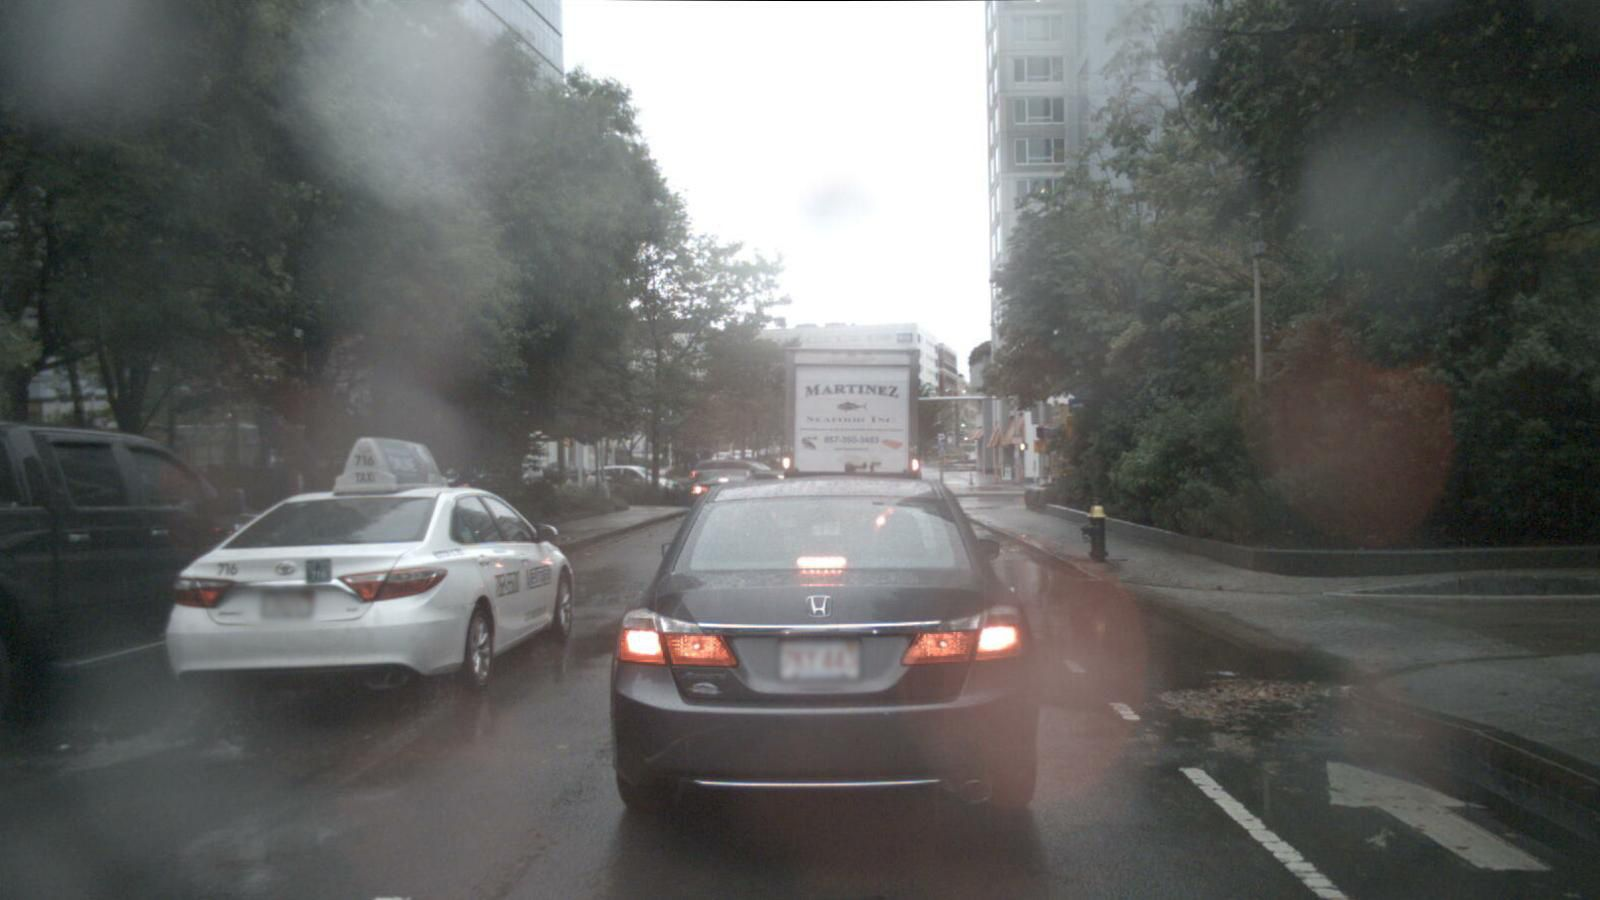
\includegraphics[width=.7\columnwidth, trim={0cm 0cm 0cm 0cm},clip]{fig/additional_nuscenes_results/rainy_scene/gt_img.png}}&
		 \raisebox{-0.5\height}{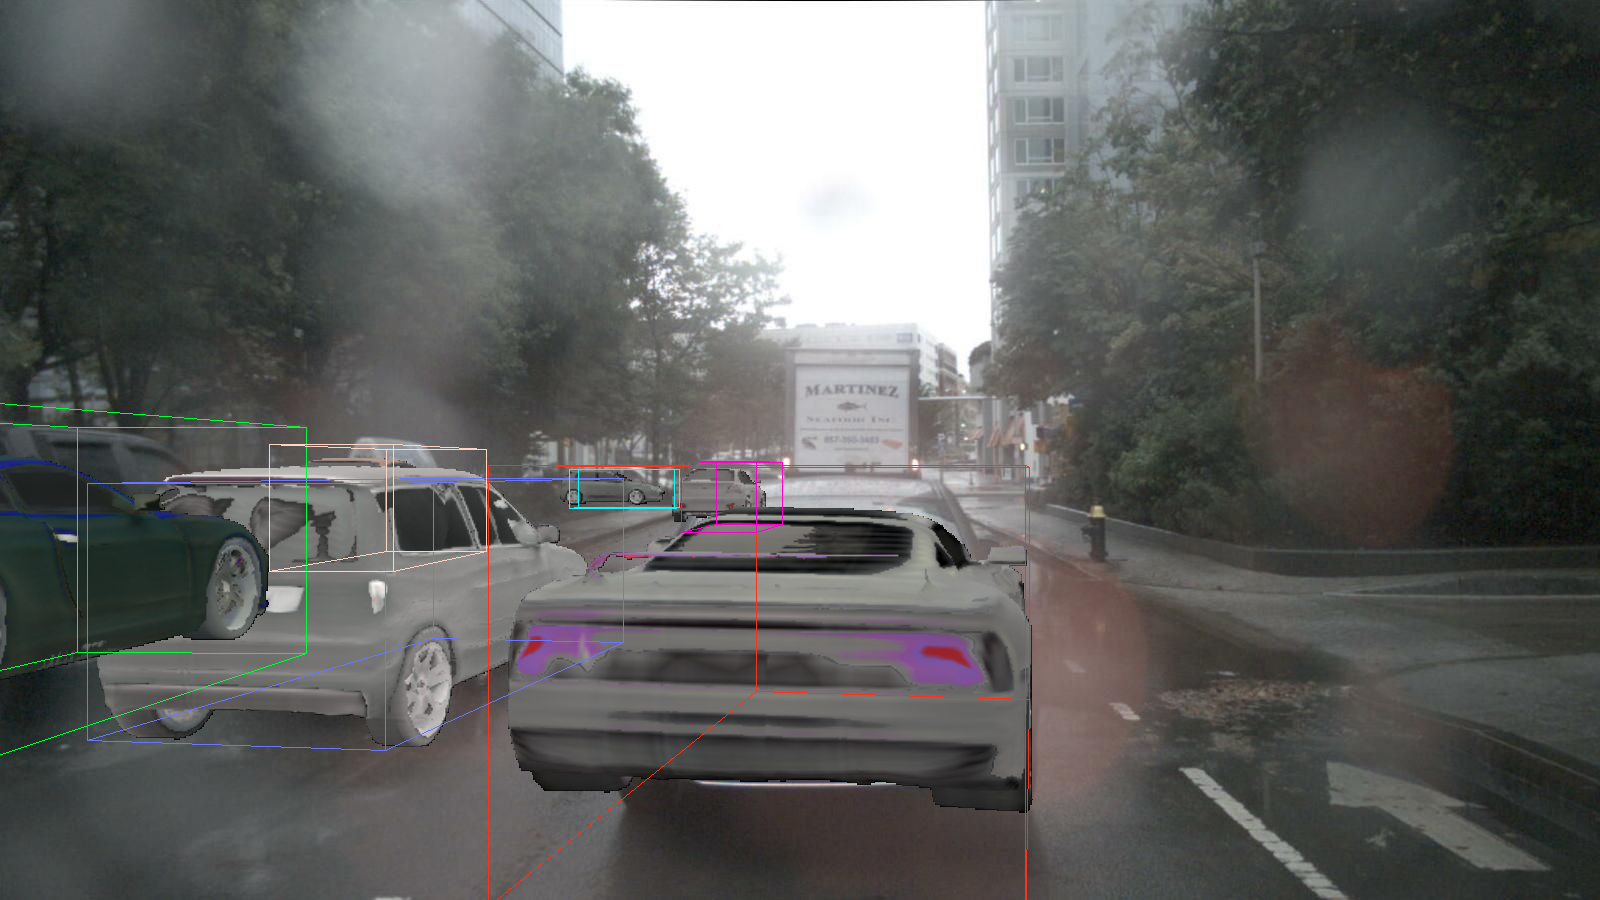
\includegraphics[width=.7\columnwidth, trim={0cm 0cm 0cm 0cm},clip]{fig/additional_nuscenes_results/rainy_scene/30.png}}&
		 \raisebox{-0.5\height}{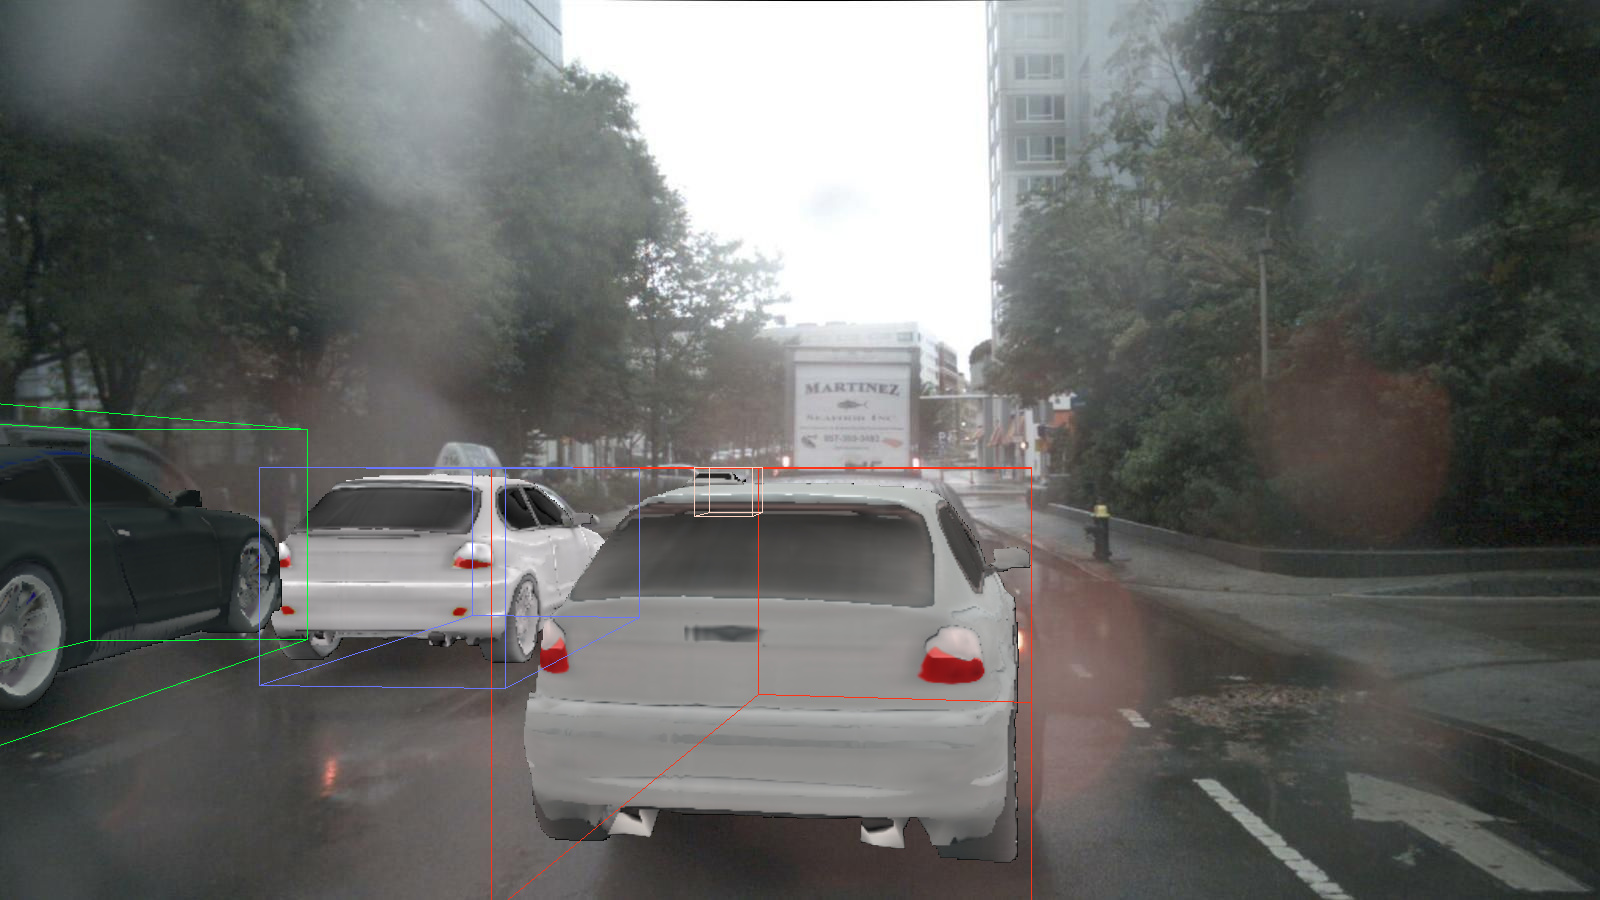
\includegraphics[width=.7\columnwidth, trim={0cm 0cm 0cm 0cm},clip]{fig/additional_nuscenes_results/rainy_scene/31.png}}&
		 % \raisebox{-0.5\height}{
\includegraphics[width=.38\columnwidth, trim={0cm 0cm 0cm 0cm},clip]{fig/placeholder-img.png}}&
		 % \raisebox{-0.5\height}{
\includegraphics[width=.38\columnwidth, trim={0cm 0cm 0cm 0cm},clip]{fig/placeholder-img.png}}
   \\[0.02cm]

   		\rotatebox[origin=c]{90}{{\Large \textbf{(e)} Det. Accuracy}}&
		\raisebox{-0.5\height}{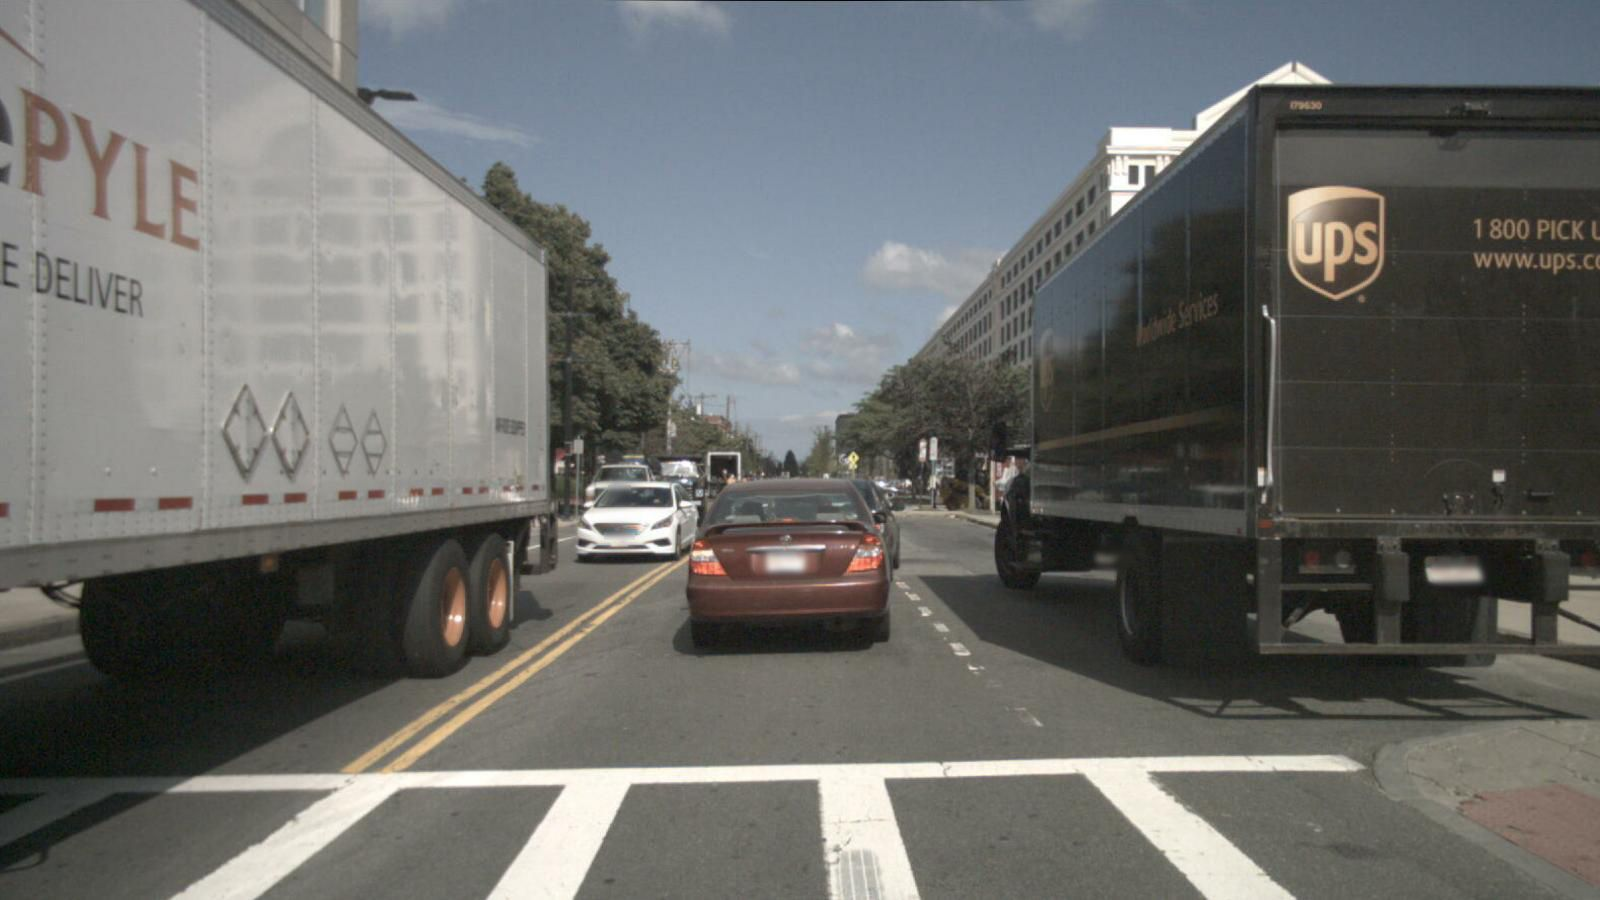
\includegraphics[width=.7\columnwidth, trim={0cm 0cm 0cm 0cm},clip]{fig/additional_nuscenes_results/scene2/2_gt.png}}&
		\raisebox{-0.5\height}{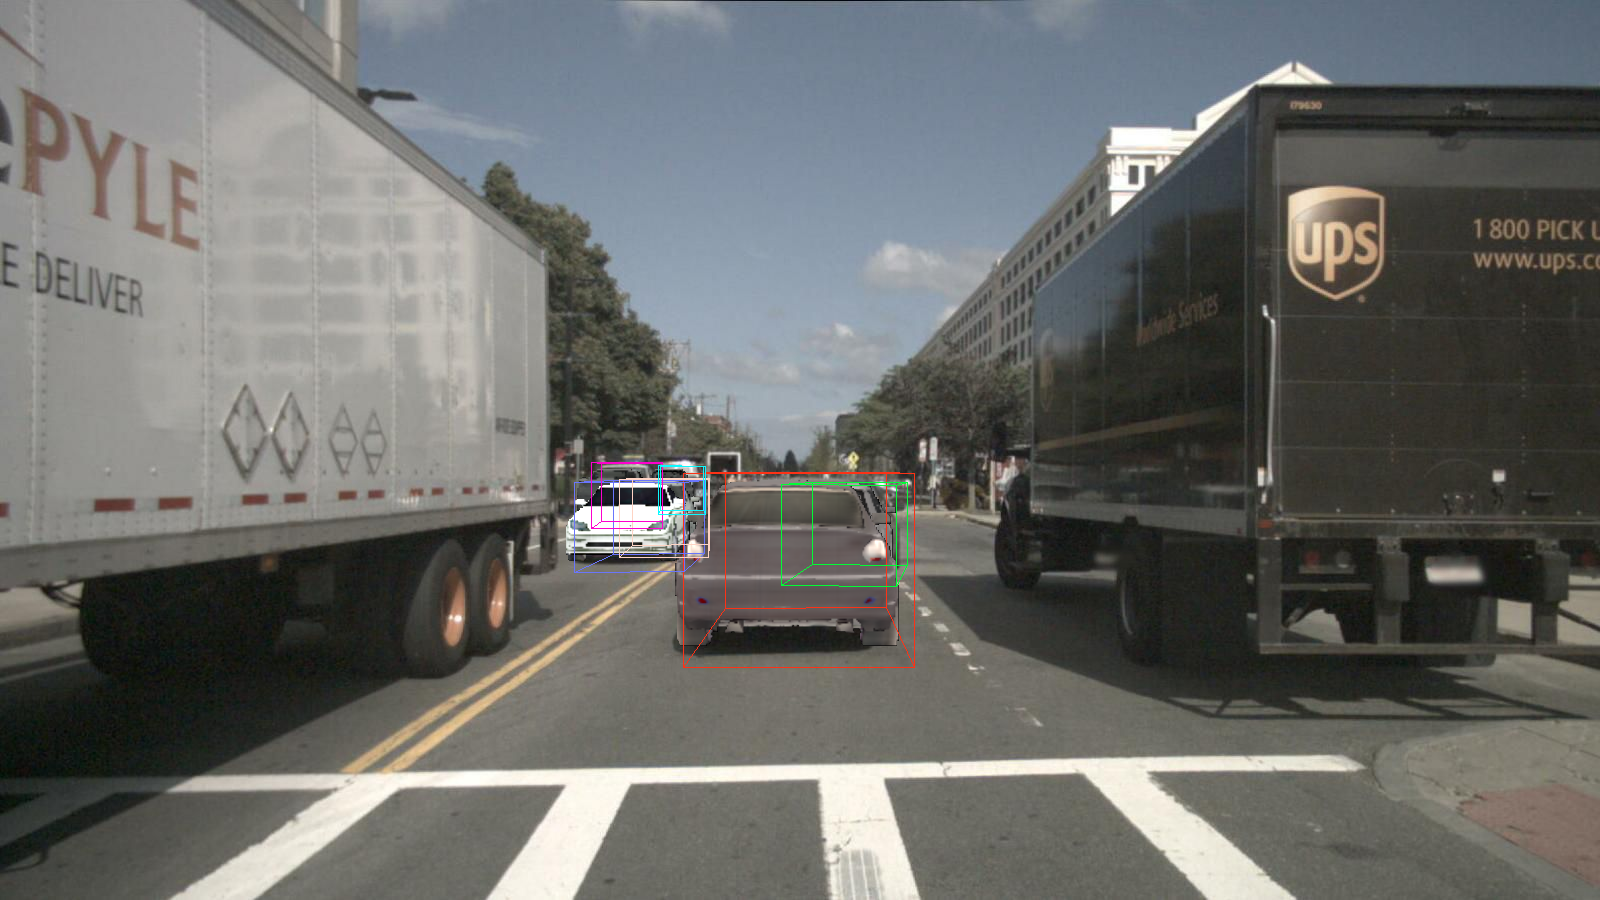
\includegraphics[width=.7\columnwidth, trim={0cm 0cm 0cm 0cm},clip]{fig/additional_nuscenes_results/scene2/2)bbix.png}} &
		\raisebox{-0.5\height}{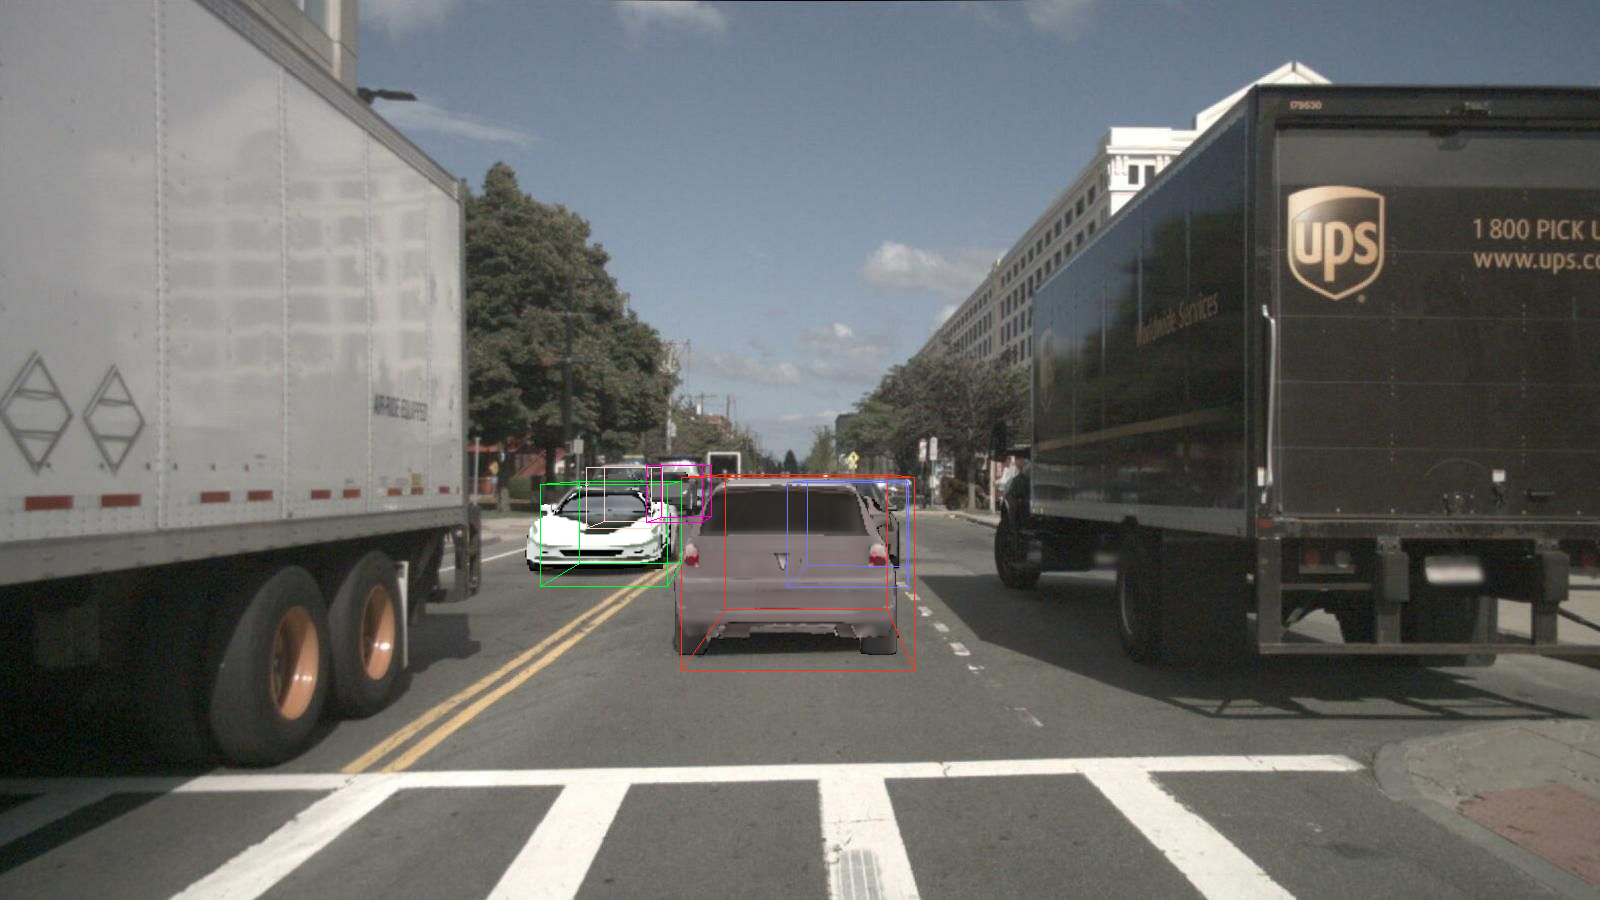
\includegraphics[width=.7\columnwidth, trim={0cm 0cm 0cm 0cm},clip]{fig/additional_nuscenes_results/scene2/3_bbox.png}}&
		% \raisebox{-0.5\height}{
\includegraphics[width=.38\columnwidth, trim={0cm 0cm 0cm 0cm},clip]{fig/placeholder-img.png}}&
		% \raisebox{-0.5\height}{
\includegraphics[width=.38\columnwidth, trim={0cm 0cm 0cm 0cm},clip]{fig/placeholder-img.png}}
\end{tabular}}
\caption{Examples of failure cases, such as lighting (shadows and reflections) or occluded objects, where the reconstructed object differs significantly from the observed object. These visualizations allow us to understand exactly why our model fails at reconstructing and tracking objects. This also allows us to identify ways the representation model and perception pipeline can be improved to incorporate effects that cause the method to fail.}
	\label{fig:interpretability}
 \end{figure}
% \end{wrapfigure}



In general, our generative prior does not model specular textures and instead is restricted to diffuse reflectance. As such, it tends to reconstruct darker or lighter textures compensating for shadows from the environment and reflections of the sky. Modeling environmental lighting, complex material properties, and shadows may lead to a complex and less robust light simulation and will be restricted by the data available to train a generative prior model. Nevertheless, this is an exciting direction for future work.

% \newpage
% % \begin{wrapfigure}{r}{0.6\linewidth}
\begin{figure}[bt!]
	\centering
\resizebox{1.\linewidth}{!}{
\renewcommand{\arraystretch}{0.5}
\begin{tabular}{@{}c@{\hskip 0.05cm}c@{\hskip 0.05cm}c@{\hskip 0.05cm}c@{}}
		\space
            &
		{\huge Input $t_0$}&
		{\huge Tracked $t_0$}&
		{\huge Tracked $t_1$}&
		% {\small Tracked $t_2$}&
		% {\small Tracked $t_3$}\\

   %           \rotatebox[origin=c]{90}{{\large  Similar colored cars}}&
		 % \raisebox{-0.5\height}{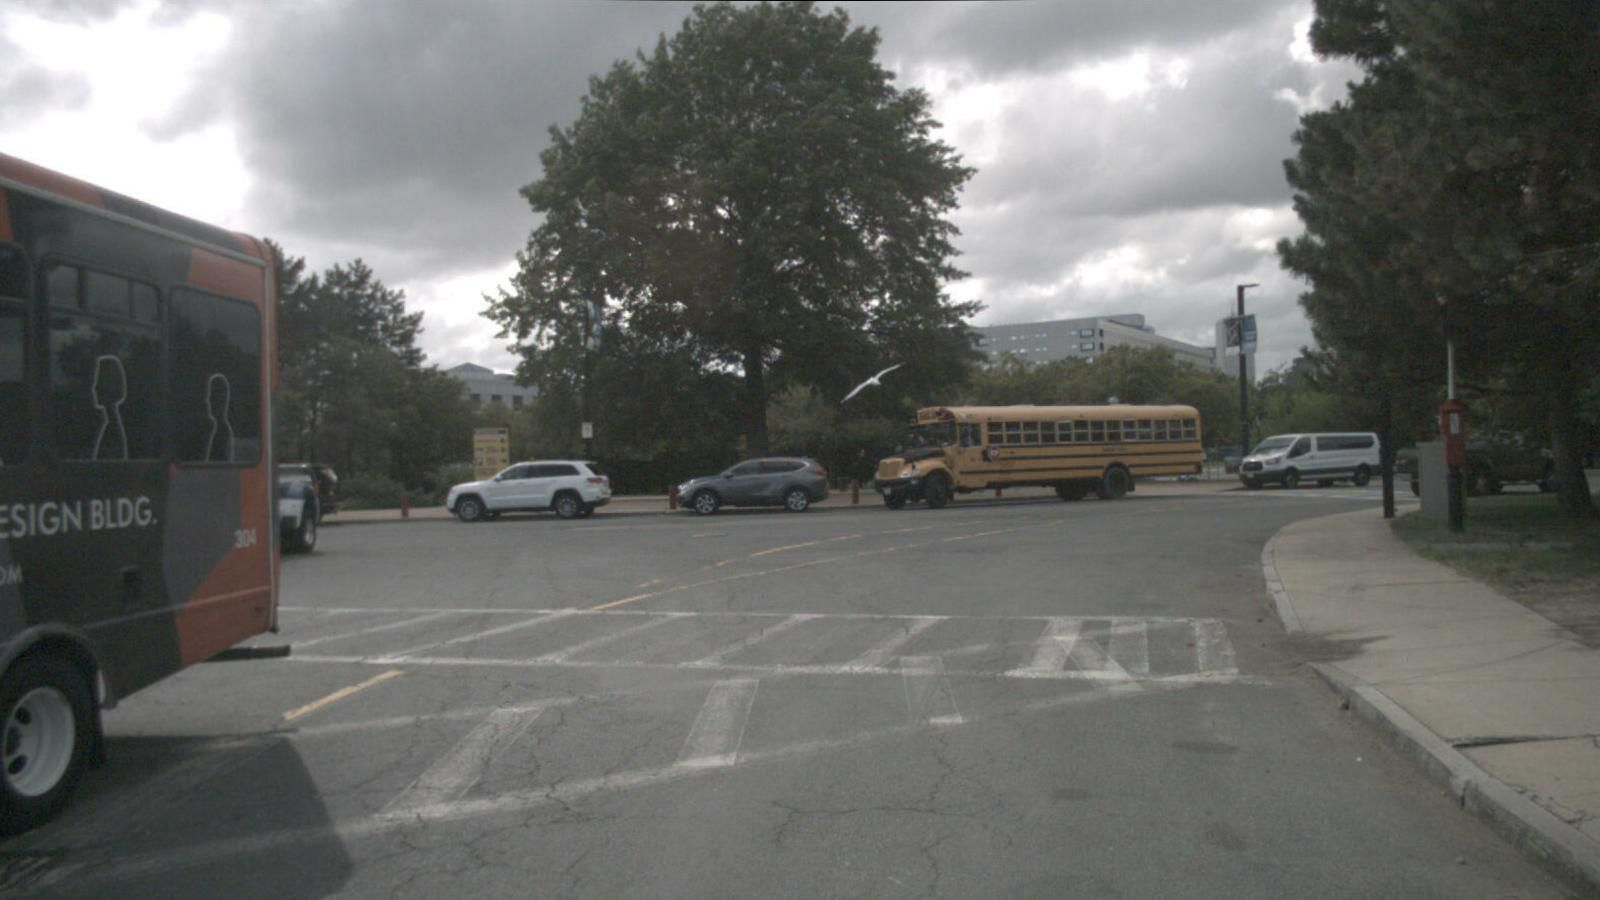
\includegraphics[width=.38\columnwidth, trim={0cm 0cm 0cm 0cm},clip]{fig/additional_nuscenes_results/scene1/26_gt.png}}&
		 % \raisebox{-0.5\height}{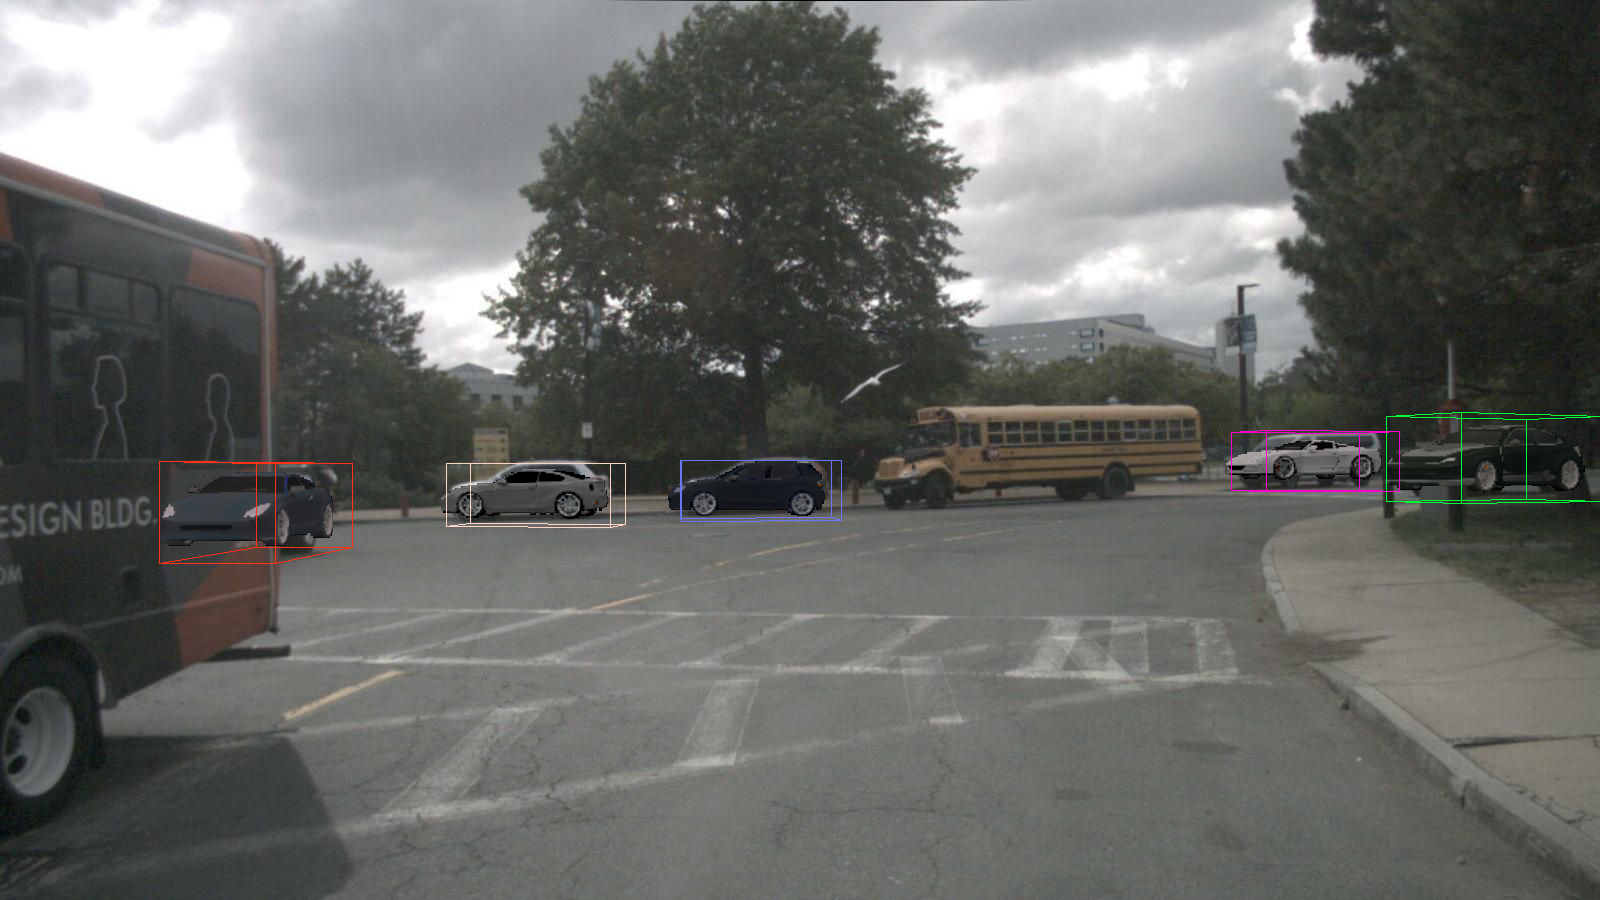
\includegraphics[width=.38\columnwidth, trim={0cm 0cm 0cm 0cm},clip]{fig/additional_nuscenes_results/scene1/26_bbox.png}}&
		 % \raisebox{-0.5\height}{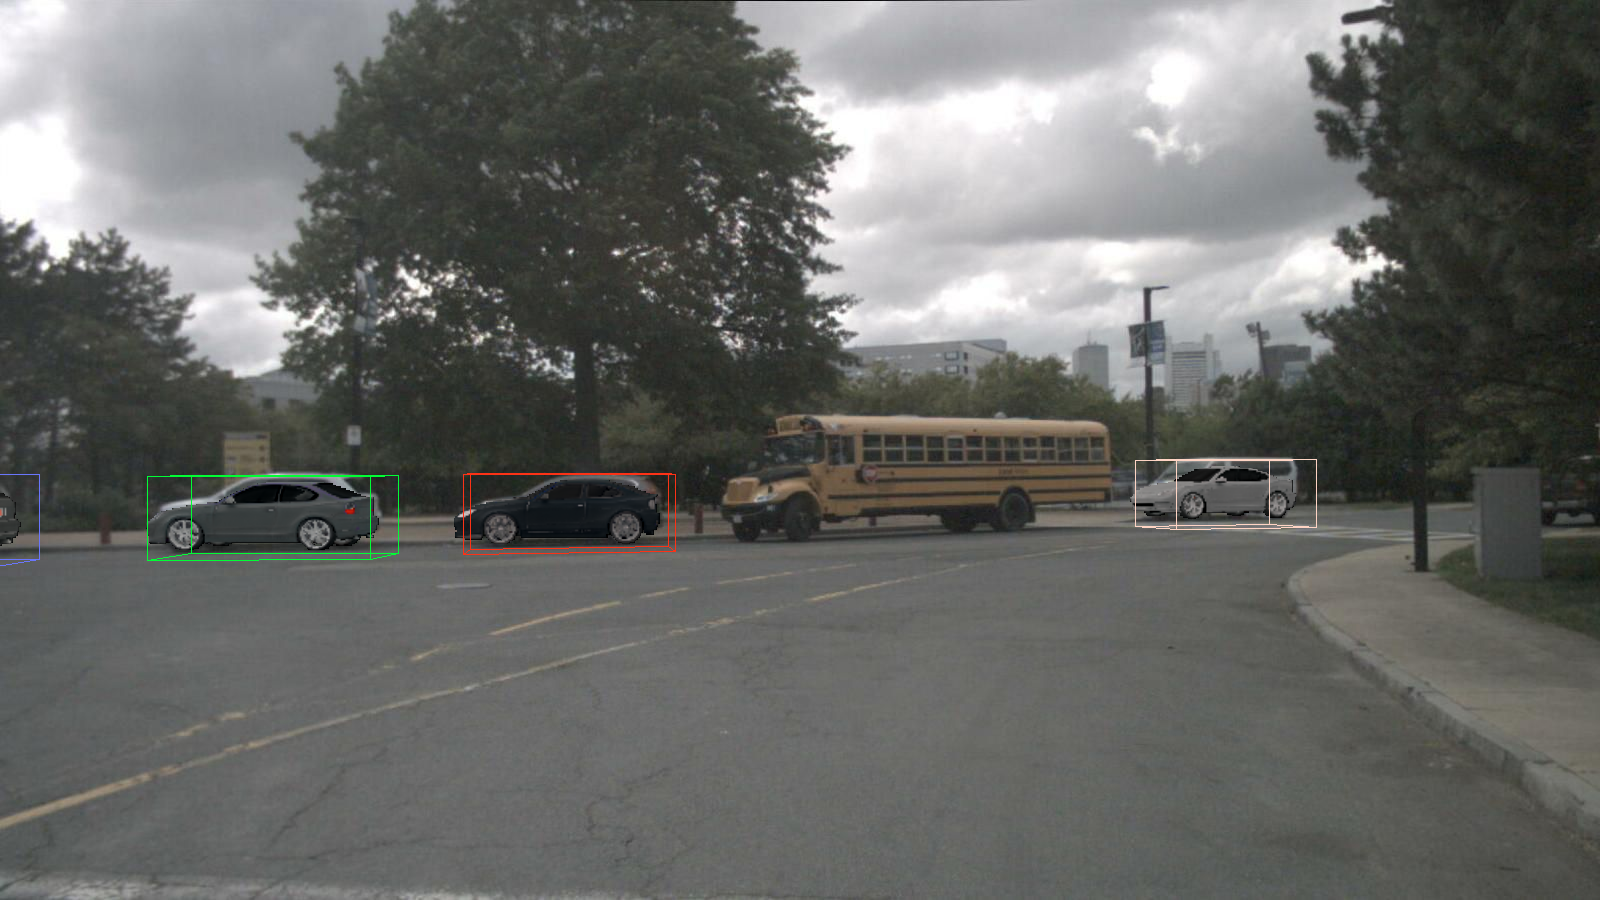
\includegraphics[width=.38\columnwidth, trim={0cm 0cm 0cm 0cm},clip]{fig/additional_nuscenes_results/scene1/28_bbox.png}}&
		 % \raisebox{-0.5\height}{
\includegraphics[width=.38\columnwidth, trim={0cm 0cm 0cm 0cm},clip]{fig/placeholder-img.png}}&
		 % \raisebox{-0.5\height}{
\includegraphics[width=.38\columnwidth, trim={0cm 0cm 0cm 0cm},clip]{fig/placeholder-img.png}}\\[0.95cm]

           \rotatebox[origin=c]{90}{{\Large \textbf{(a)} Shadow}}&
  		\raisebox{-0.5\height}{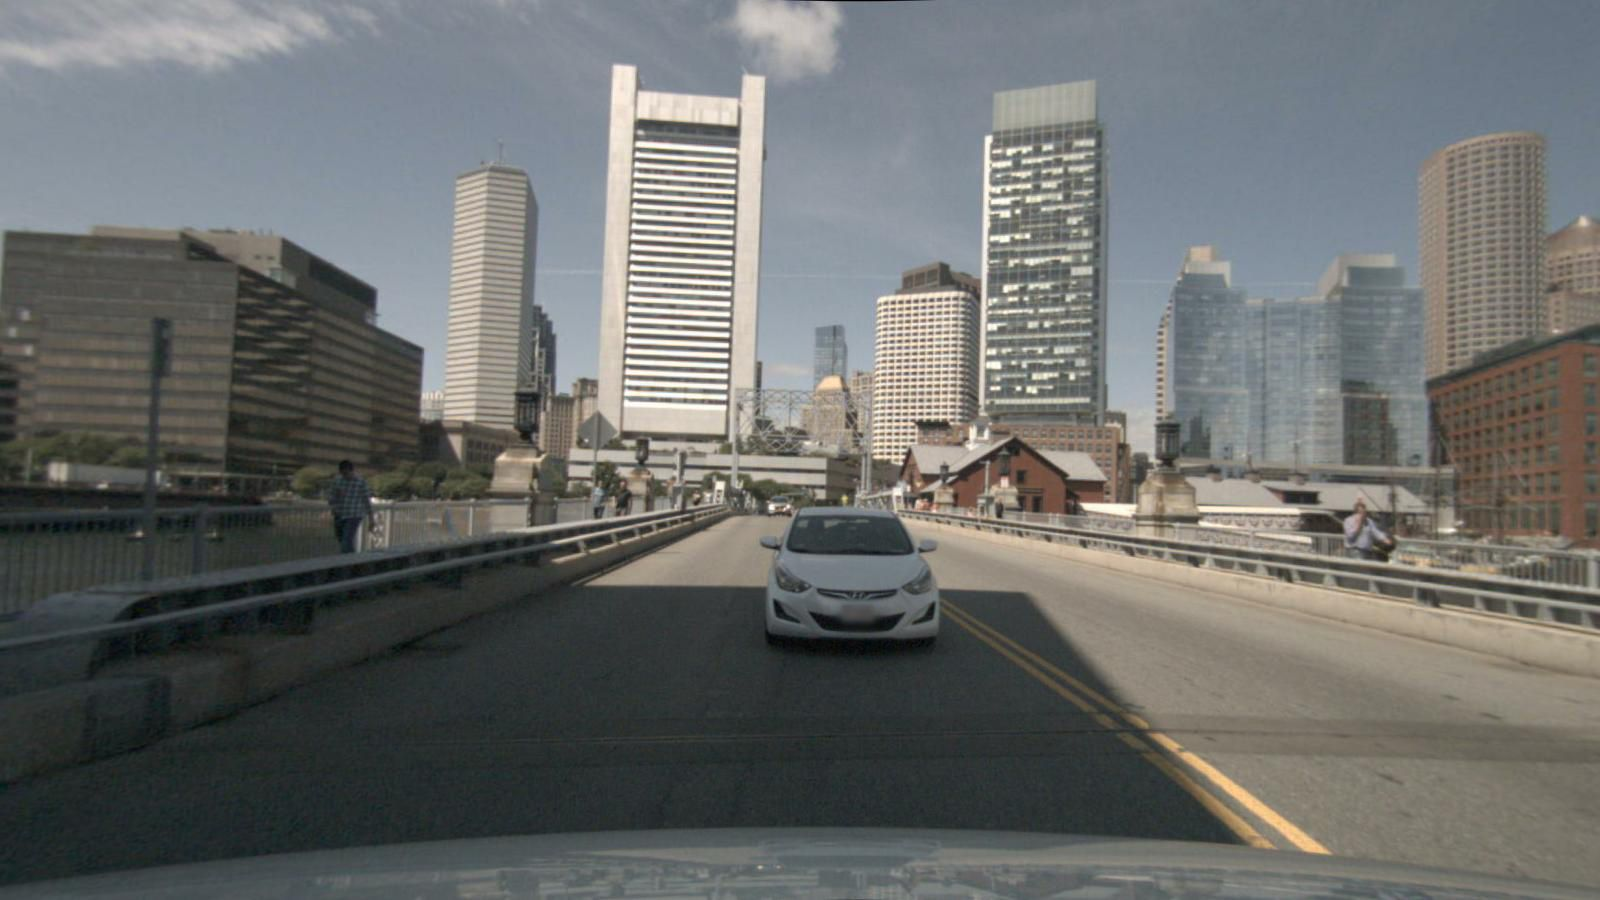
\includegraphics[width=.7\columnwidth, trim={0cm 0cm 0cm 0cm},clip]{fig/additional_nuscenes_results/scene12/gt.png}}&
		\raisebox{-0.5\height}{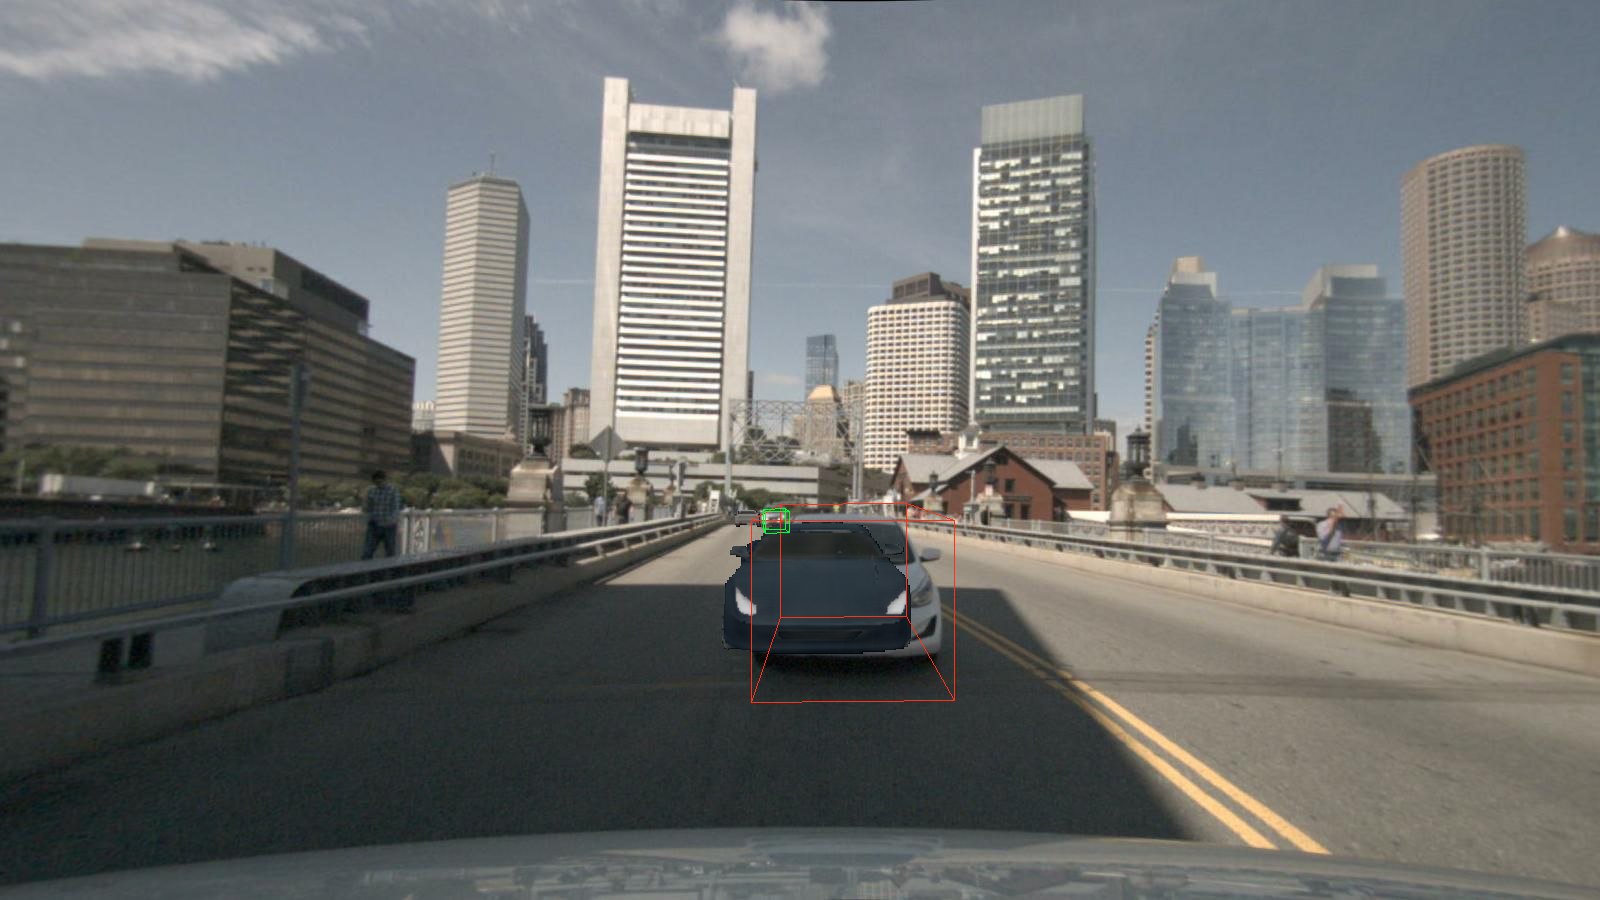
\includegraphics[width=.7\columnwidth, trim={0cm 0cm 0cm 0cm},clip]{fig/additional_nuscenes_results/scene12/21.png}}&
		\raisebox{-0.5\height}{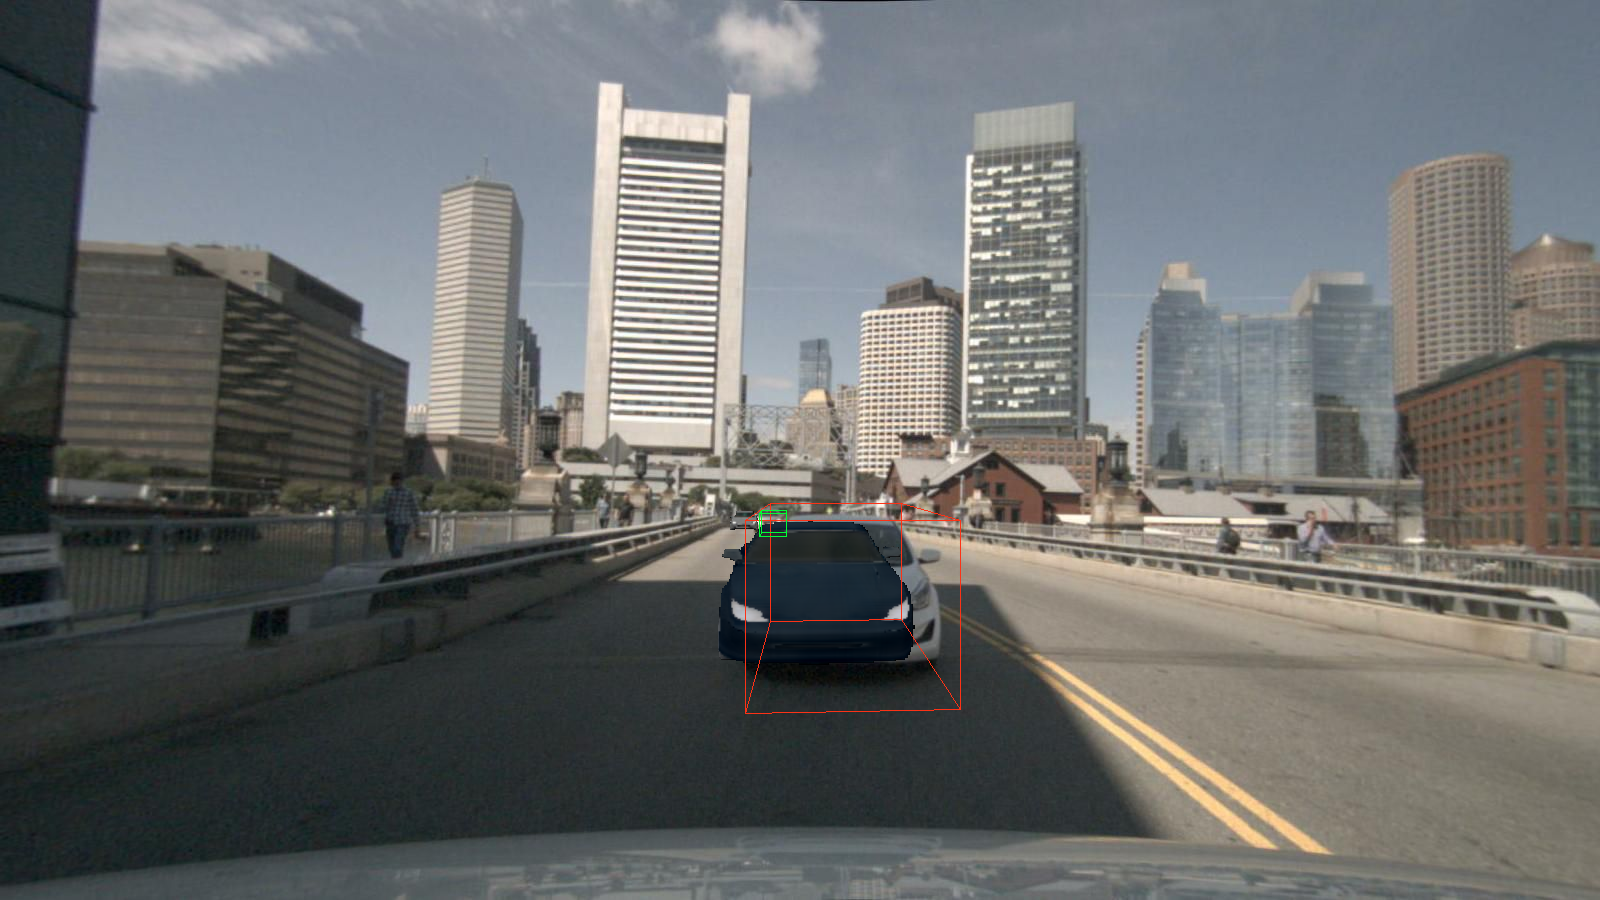
\includegraphics[width=.7\columnwidth, trim={0cm 0cm 0cm 0cm},clip]{fig/additional_nuscenes_results/scene12/22.png}}&
		% \raisebox{-0.5\height}{
\includegraphics[width=.38\columnwidth, trim={0cm 0cm 0cm 0cm},clip]{fig/placeholder-img.png}}&
		% \raisebox{-0.5\height}{
\includegraphics[width=.38\columnwidth, trim={0cm 0cm 0cm 0cm},clip]{fig/placeholder-img.png}}
  \\[0.02cm]

            \rotatebox[origin=c]{90}{{\Large \textbf{(b)} Reflection}}&
  		\raisebox{-0.5\height}{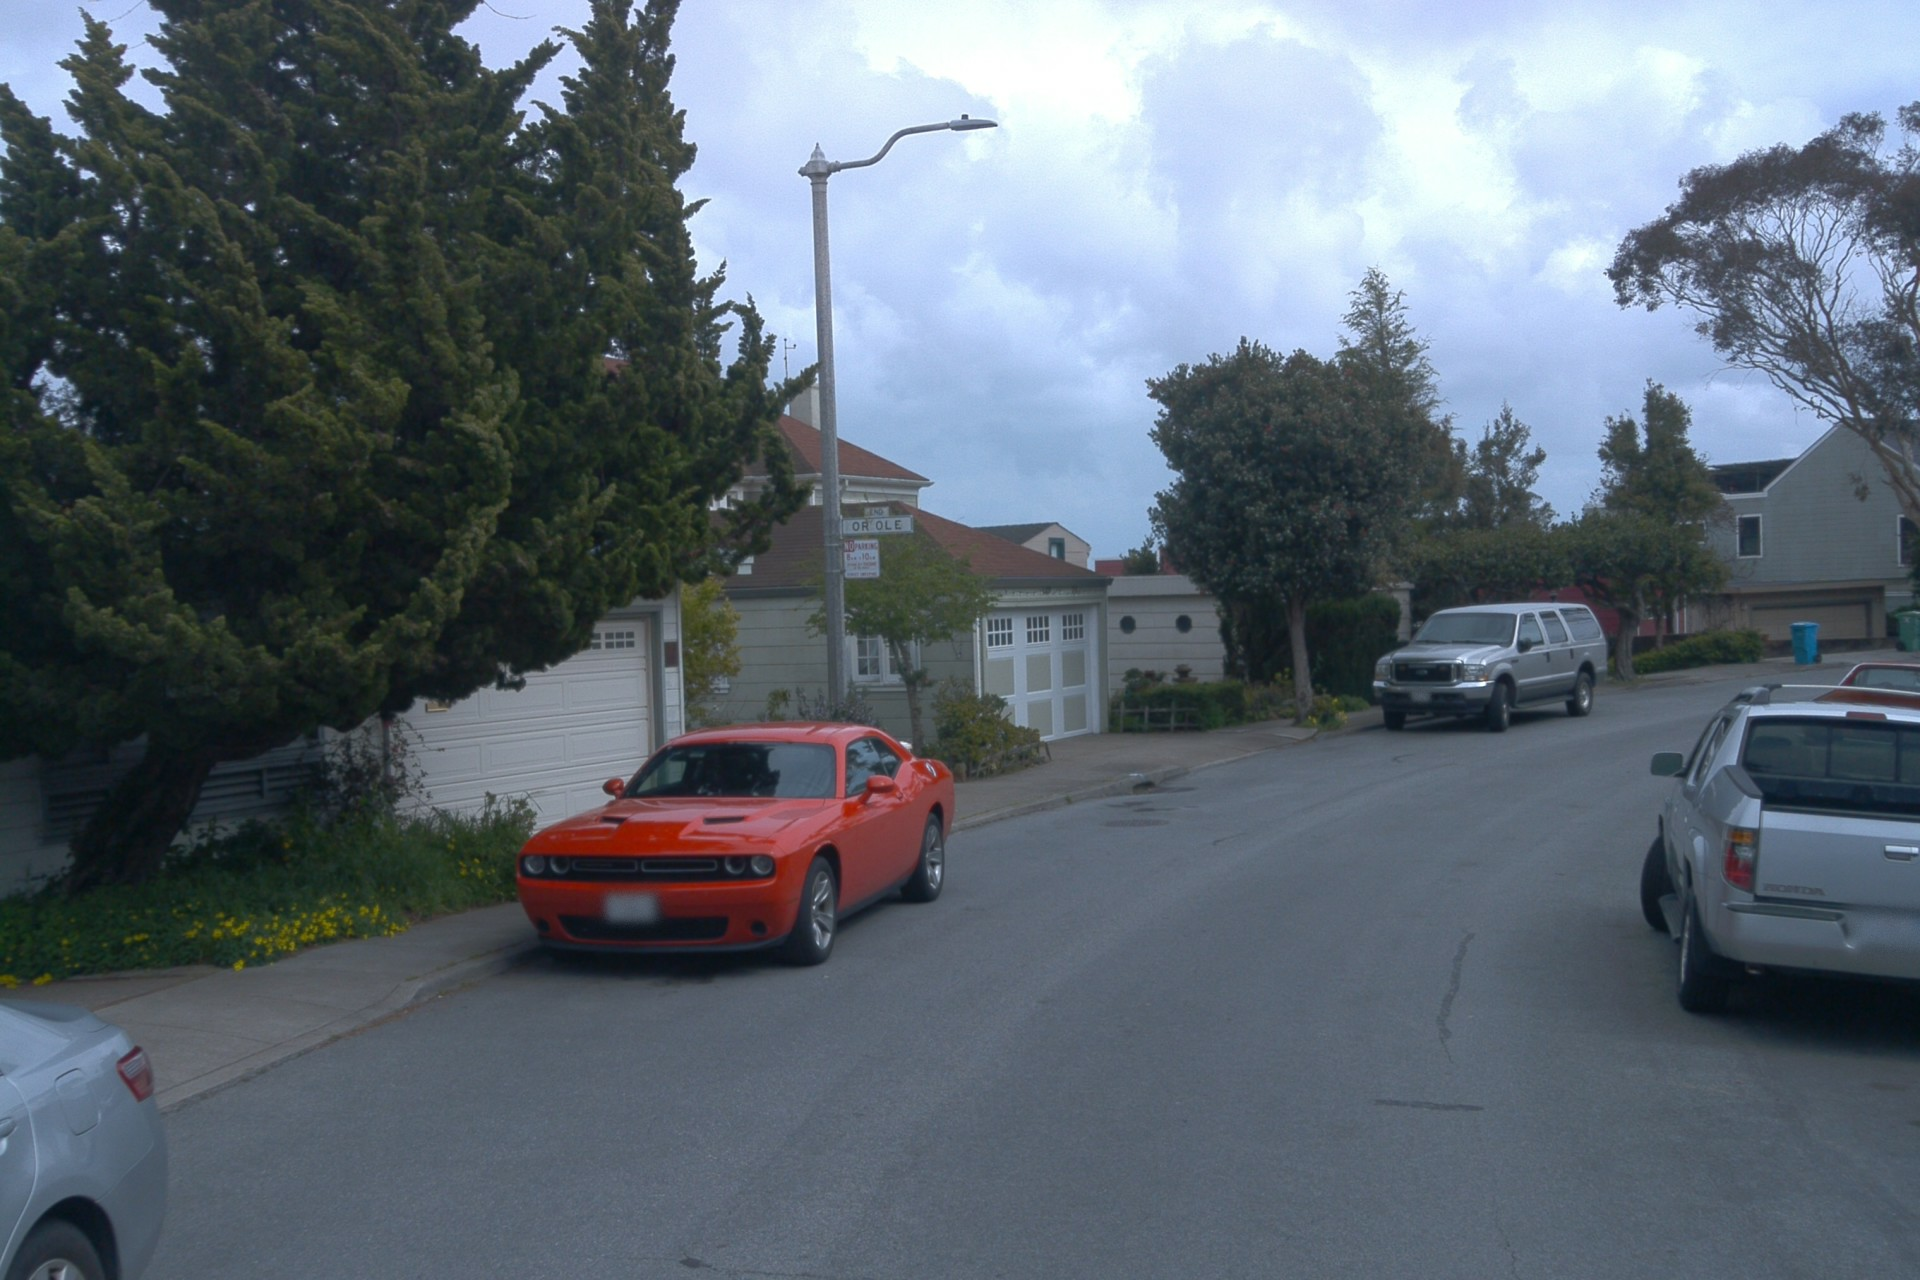
\includegraphics[width=.7\columnwidth, trim={0cm 0cm 0cm 0cm},clip]{fig/additional_waymo_results/scene4/gt_img.png}}&
		\raisebox{-0.5\height}{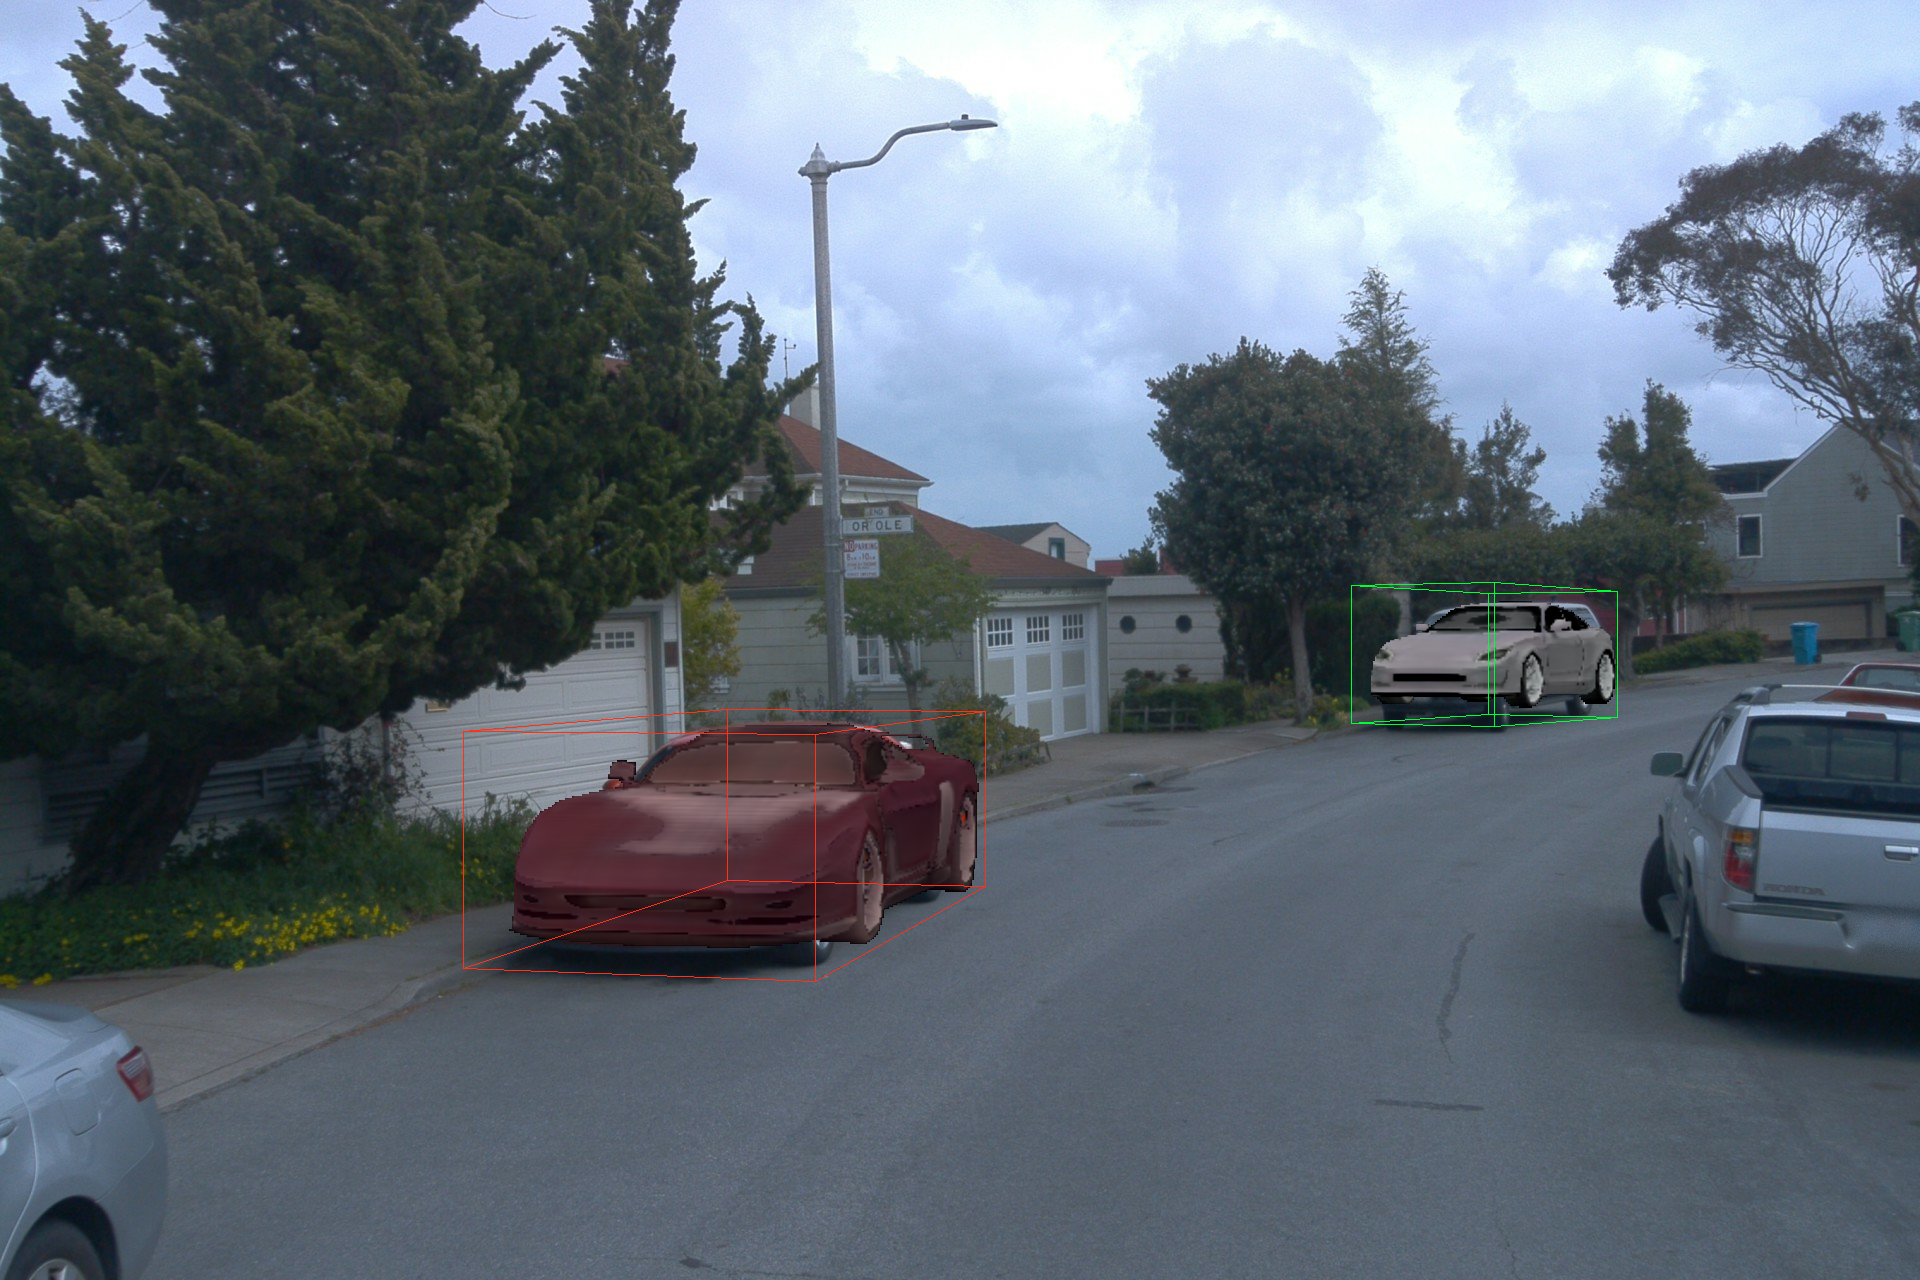
\includegraphics[width=.7\columnwidth, trim={0cm 0cm 0cm 0cm},clip]{fig/additional_waymo_results/scene4/5.png}}&
		\raisebox{-0.5\height}{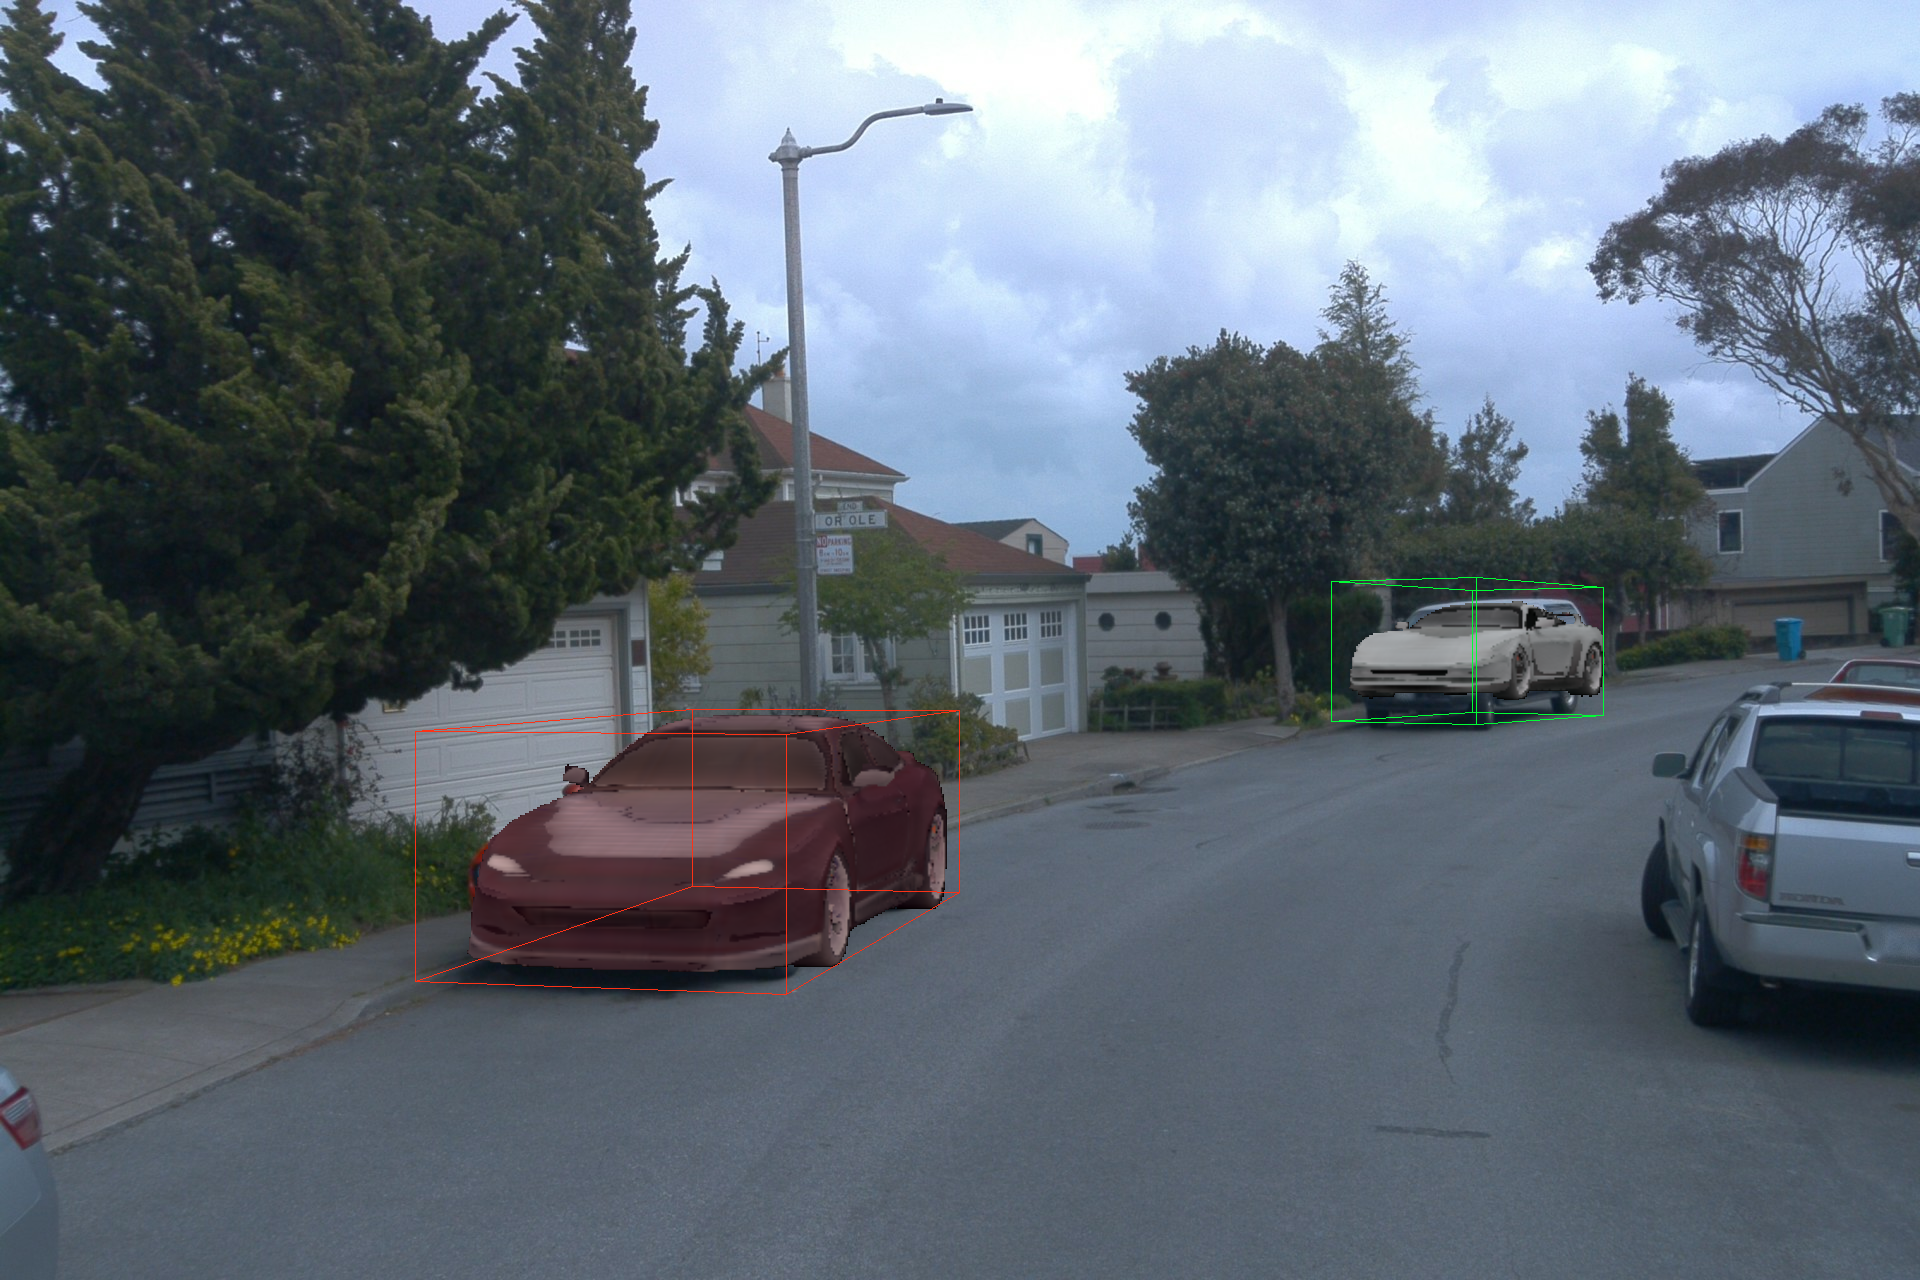
\includegraphics[width=.7\columnwidth, trim={0cm 0cm 0cm 0cm},clip]{fig/additional_waymo_results/scene4/6.png}}&
		% \raisebox{-0.5\height}{
\includegraphics[width=.38\columnwidth, trim={0cm 0cm 0cm 0cm},clip]{fig/placeholder-img.png}}&
		% \raisebox{-0.5\height}{
\includegraphics[width=.38\columnwidth, trim={0cm 0cm 0cm 0cm},clip]{fig/placeholder-img.png}}
  \\[0.02cm]
  
           \rotatebox[origin=c]{90}{{\Large \textbf{(c)} Occlusion}}&
		 \raisebox{-0.5\height}{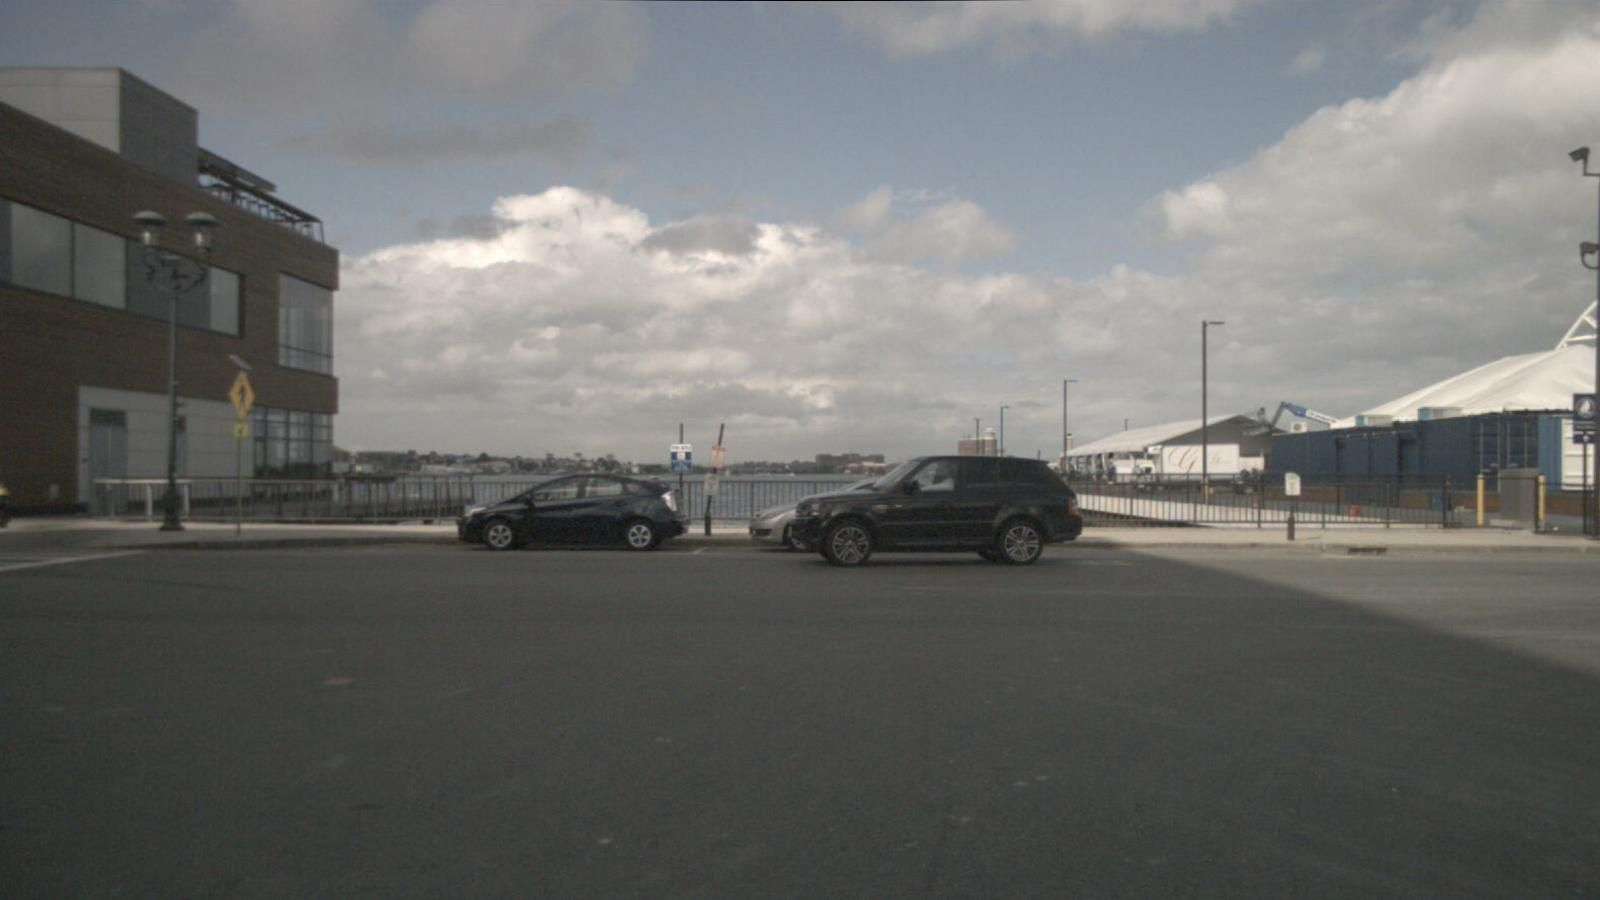
\includegraphics[width=.7\columnwidth, trim={0cm 0cm 0cm 0cm},clip]{fig/additional_nuscenes_results/scene7/0118_4_gt.png}}&
		 \raisebox{-0.5\height}{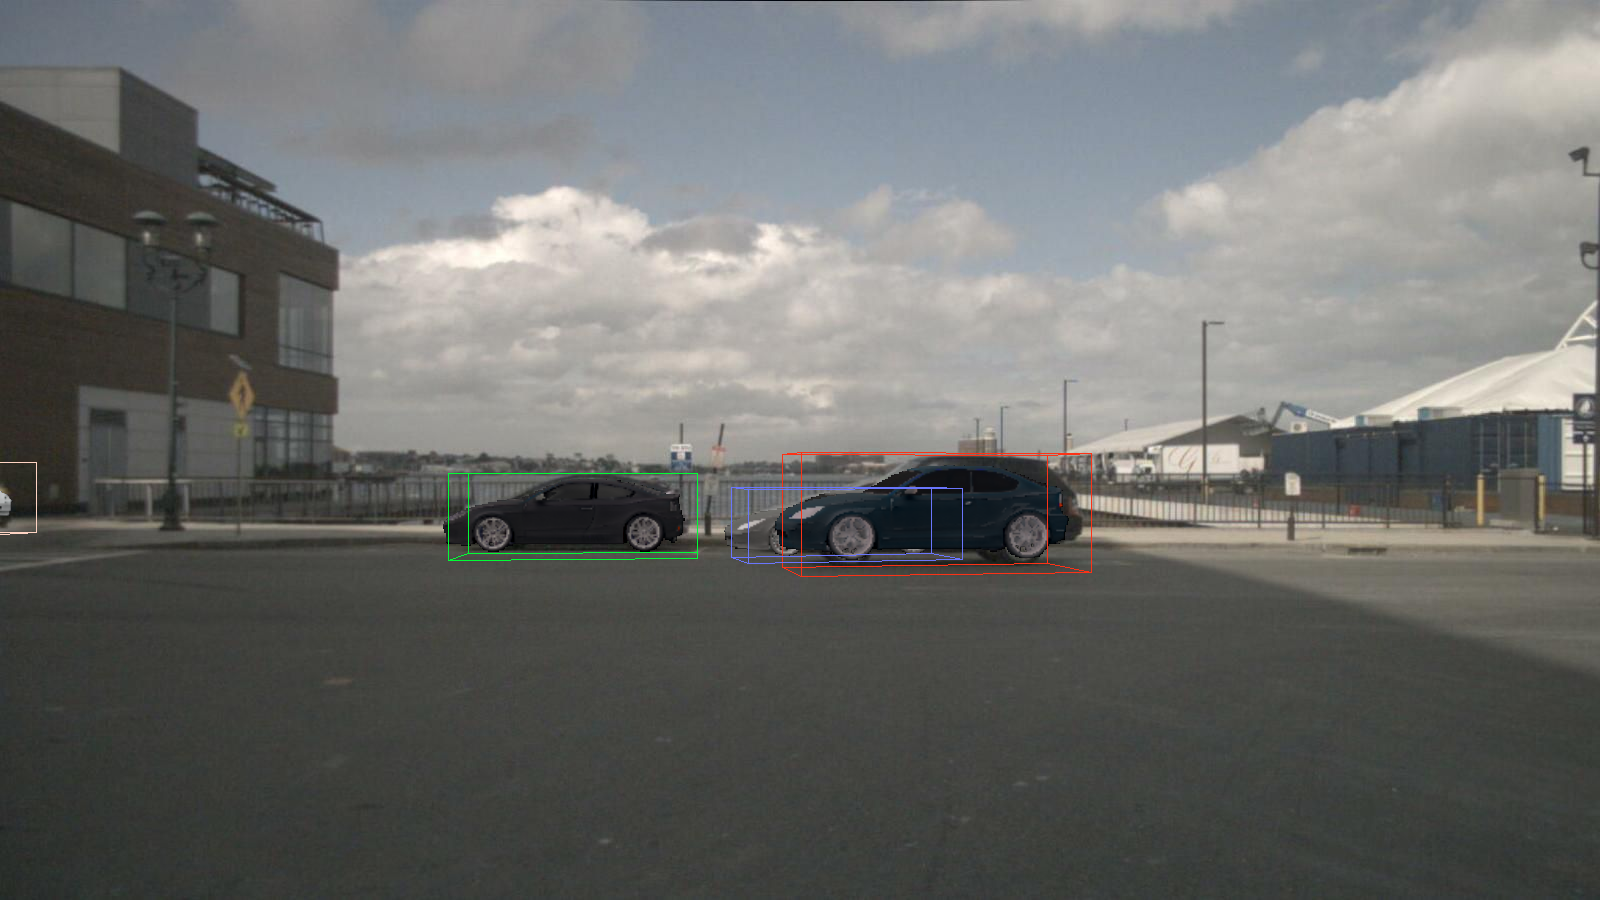
\includegraphics[width=.7\columnwidth, trim={0cm 0cm 0cm 0cm},clip]{fig/additional_nuscenes_results/scene7/0118_4_bbox.png}}&
		 \raisebox{-0.5\height}{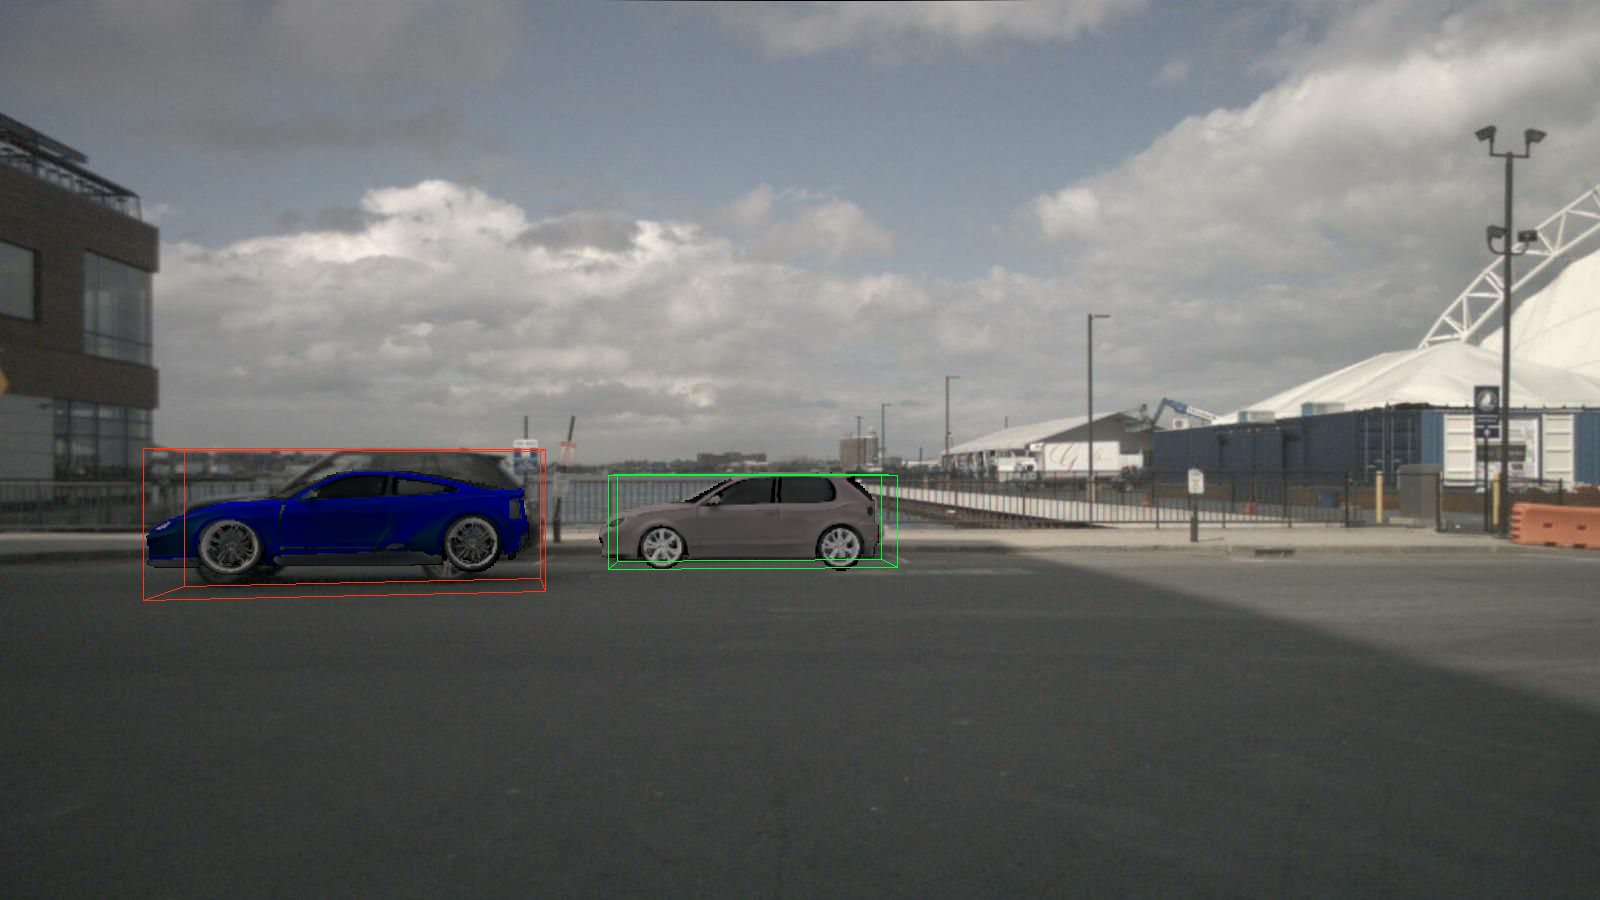
\includegraphics[width=.7\columnwidth, trim={0cm 0cm 0cm 0cm},clip]{fig/additional_nuscenes_results/scene7/0118_6_bbox.png}}&
		 % \raisebox{-0.5\height}{
\includegraphics[width=.38\columnwidth, trim={0cm 0cm 0cm 0cm},clip]{fig/placeholder-img.png}}&
		 % \raisebox{-0.5\height}{
\includegraphics[width=.38\columnwidth, trim={0cm 0cm 0cm 0cm},clip]{fig/placeholder-img.png}}
   \\[0.02cm]
        
        \rotatebox[origin=c]{90}{{\Large \textbf{(d)} Obstruction}}&
		 \raisebox{-0.5\height}{\includegraphics[width=.7\columnwidth, trim={0cm 0cm 0cm 0cm},clip]{fig/additional_nuscenes_results/rainy_scene/gt_img.png}}&
		 \raisebox{-0.5\height}{\includegraphics[width=.7\columnwidth, trim={0cm 0cm 0cm 0cm},clip]{fig/additional_nuscenes_results/rainy_scene/30.png}}&
		 \raisebox{-0.5\height}{\includegraphics[width=.7\columnwidth, trim={0cm 0cm 0cm 0cm},clip]{fig/additional_nuscenes_results/rainy_scene/31.png}}&
		 % \raisebox{-0.5\height}{\includegraphics[width=.38\columnwidth, trim={0cm 0cm 0cm 0cm},clip]{fig/placeholder-img.png}}&
		 % \raisebox{-0.5\height}{\includegraphics[width=.38\columnwidth, trim={0cm 0cm 0cm 0cm},clip]{fig/placeholder-img.png}}
   \\[0.02cm]

   		\rotatebox[origin=c]{90}{{\Large \textbf{(e)} Det. Accuracy}}&
		\raisebox{-0.5\height}{\includegraphics[width=.7\columnwidth, trim={0cm 0cm 0cm 0cm},clip]{fig/additional_nuscenes_results/scene2/2_gt.png}}&
		\raisebox{-0.5\height}{\includegraphics[width=.7\columnwidth, trim={0cm 0cm 0cm 0cm},clip]{fig/additional_nuscenes_results/scene2/2)bbix.png}} &
		\raisebox{-0.5\height}{\includegraphics[width=.7\columnwidth, trim={0cm 0cm 0cm 0cm},clip]{fig/additional_nuscenes_results/scene2/3_bbox.png}}&
		% \raisebox{-0.5\height}{\includegraphics[width=.38\columnwidth, trim={0cm 0cm 0cm 0cm},clip]{fig/placeholder-img.png}}&
		% \raisebox{-0.5\height}{\includegraphics[width=.38\columnwidth, trim={0cm 0cm 0cm 0cm},clip]{fig/placeholder-img.png}}
\end{tabular}}
\caption{Examples of failure cases, such as lighting (shadows and reflections) or occluded objects, where the reconstructed object differs significantly from the observed object. These visualizations allow us to understand exactly why our model fails at reconstructing and tracking objects. This also allows us to identify ways the representation model and perception pipeline can be improved to incorporate effects that cause the method to fail.}
	\label{fig:interpretability}
 \end{figure}
% \end{wrapfigure}

% \newpage

% \todo{The rendered output images provide interpretable inference results that explain successful or failed matching due to shadows, appearance, shape, or pose. For example, the blue car in the IR inference in Fig. 5 top row was incorrectly matched due to an appearance mismatch in a shadow region. A rendering model including ambient illumination may resolve this ambiguity, see further discussion in the Supplementary Material.}